\documentclass[12pt]{article}

\usepackage[
  backend=biber,
  style=numeric,      % or another style: 'authoryear', 'alphabetic', etc.
  backref=true,
  backrefstyle=three  % optional: shows "Cited on pages..." nicely
]{biblatex}

\addbibresource{references.bib}

\usepackage{setspace} % Line spacing control
\setstretch{1.1}     % Line spacing set to 1.1 (slightly tighter than 1.5)

\usepackage{amssymb}
\usepackage{hyperref}
\usepackage[utf8]{inputenc}
\usepackage{tcolorbox}
\usepackage{amsmath}
\usepackage{amsthm}
\usepackage{enumitem}
\usepackage{bm}
\usepackage{algorithm}
\usepackage{algorithmic}
\usepackage{float}
\usepackage{parskip}
\usepackage{tikz}
\usetikzlibrary{graphs, shapes, positioning}
\usetikzlibrary{backgrounds}
\usetikzlibrary{positioning}

\usepackage[margin=0.5in]{geometry} % Uniform 1-inch margins

\usepackage{fancyhdr} 
\pagestyle{fancy}     
\lhead{}              
\chead{}
\rhead{\thepage}
\lfoot{}
\cfoot{}
\rfoot{}

\usepackage{titlesec}  % For section title customization
\titleformat{\section}[block]{\normalfont\huge\bfseries}{\thesection}{1em}{}
\titleformat{\subsection}[block]{\normalfont\large\bfseries}{\thesubsection}{1em}{}

\usepackage{listings}  % For better code formatting
\lstset{
  basicstyle=\ttfamily\footnotesize,
  numbers=left,
  numberstyle=\tiny,
  stepnumber=1,
  numbersep=5pt,
  backgroundcolor=\color{gray!10},
  frame=single,
  captionpos=b
}


\setlength{\parskip}{0.5em}

\hbadness=10000
\hfuzz=50pt

\newcounter{definition}[section] % Reset the counter at every new section
\renewcommand{\thedefinition}{\thesection.\arabic{definition}} % Format the counter as section.definition

\newtcolorbox[]{mydefinition}[2][]{%
  colback=blue!5!white,  % Background color
  colframe=blue!75!black, % Frame color
  fonttitle=\bfseries,    % Title font
  width=\textwidth,       % Box width
  sharp corners,          % Style options
  title=#2~\thedefinition: #1,  % Custom label and number
}

\title{\huge Certified Algorithms for Combinatorial Optimization Problems}
\author{\Large Martin Sokolov}
\date{\today}

\begin{document}

\maketitle

\tableofcontents

\section{Introduction}

This section introduces the topic and provides background information. 
\section{Preliminaries}

In this section, we provide the reader with the necessary information in order to follow the paper. We start 
off with a reminder on Graph Theory. After that, we move to more advanced definitions in the field of 
Combinatorial Optimization. Finally, we get more on topic by introducing perturbation resilience and certified 
algorithms from the field of Beyond the Worst-Case Analysis of Algorithms.

\subsection{Graph Theory}

In this section, the authors refer to Bondy and Murty \cite{bondy1976graph}.
From the same book we get a definition for a \textit{graph} $G$ is an ordered pair $(V(G), E(G))$.
The set $V(G)$ is called a set of \textit{vertices} and the set $E(G)$, a set of \textit{edges}.
Together with the incidence function $\psi_G$, that associates each edge with an unordered pair of 
(not necessarily unique) vertices, we define a graph $G$. We are going to use $n$ as the cardinality 
of the set $V$ and $m$ for the set of edges $E$. With each edge $e$ of G, let there be associated 
a real number $w(e)$, called its \textit{weight}. Then G, together with the weighting function 
$w : E \to \mathbb{R}$, is called a \textit{weighted graph}, and denoted $(G, w)$.

A graph is can be \textit{embedded in the plane}, or is \textit{planar} if it can be drawn on the 
plane in a way that edges intersect each other only at their ends. Such a drawing is called a 
\textit{planar embedding} of the graph. A graph $G$ is called \textit{outerplanar} if it has a 
planar embedding $\widetilde{G}$ in which all the vertices lie on the boundary of the outer face. 
This is also called a \textit{1-outerplanar graph}. Two forbidden minors of that class are the 
$K_4$ and $K_{2, 3}$ graphs. In the next subsection we familiarize the reader with Baker's approach 
\cite{Baker}. Here we define a \textit{k-outerplanar} to be a graph that has a planar embedding in which 
the vertices belong to at most $k$ concentric layers. Every planar graph is \textit{k-outerplanar} for 
some $k$. Given a graph $G$, we look for \textit{k-outerplanar} embedding of $G$ for which $k$ is minimal.
\section{(E)PTAS for FVS-BCL Problem Using Baker's Technique}

\noindent In this section we provide the necessary definitions, lemmas and theorems to demonstrate how to obtain an EPTAS for the problem 
we defined in \ref{FVS-BCL}, namely FVS-BCL. In the preliminaries we gave two examples of how to construct algorithms using Baker's technique 
and how to further analyse them. In the same fashion we now construct Algorithm \ref{alg:ufvsbcl} and reason for its effectiveness.

\noindent In the following algorithm we use the letter $\ell$ for the outerplanarity of each subgraph, i.e. each $G_{i, j}$ that we 
define on line 4 in Algorithm~\ref{alg:ufvsbcl} is $\ell$-outerplanar.

\begin{algorithm}[H]
    \caption{Baker's technique for the unweighted FVS-BCL}
    \label{alg:ufvsbcl}
    \begin{algorithmic}[1]
    \REQUIRE Planar graph $G = (V, E)$, parameter $\ell$
    \ENSURE $(1 + \epsilon)$-approximation for \textsc{FVS-BCL}
    \STATE Perform \textsc{BFS} from some arbitrary vertex $r$
    \STATE $S \leftarrow \emptyset$

    $i$: \textit{shift}; $j$: \textit{slice}

    \FOR{each $i = 0$ to $\ell-1$}
        \STATE Let $G_{i, j}$ be the subgraph induced on vertices at levels $j \times k + i$ through $(j+1) \times k + i$ for $0 \leq i < k$.
        \STATE $\forall j \text{ compute }  S_{i, j}$, the min. \textsc{VC} of $G_{i, j}$.
        \STATE $\forall j \text{ let } S_i = \bigcup_{j} S_{i, j}$
        \STATE $S \leftarrow S \cup S_i$
    \ENDFOR
    \RETURN $S_{i*}$ from $S$ with minimum cardinality
    \end{algorithmic}
\end{algorithm}

\noindent In the analysis of the algorithm we are going to need three lemmas in order 
to prove that Algorithm~\ref{alg:ufvsbcl} obtains a $(1 + 2/\ell)$-approximation of the 
optimum solution.

\refstepcounter{definition}
\begin{mydefinition}[Optimum solution bound]{Lemma}
    \label{lemma-one}

    Let $S_{i, j}$ be an optimum solution for $G_{i, j}$ for some shift $i$ and slice $j$, 
    let $F \equiv OPT$ be the optimum solution in $G$ and let $F_{i, j} = G_{i, j} \cap F$. 
    In the unweighted case we claim that: \[|S_{i, j}| \leq |F_{i, j}|\text{.}\]

    We will say that $F_{i, j}$ is a FVS-BCL of $G_{i, j}$, not necessarily the one of minimum cardinality.

\end{mydefinition}

\noindent For now we do not argue about how we obtain an optimum solution, in further sections we will show how 
to to get it using tree decompositions and dynamic programming, but for now we argue that this inequality 
holds in each subgraph $G_{i, j}$.

\noindent We first argue that in each subgraph $G_{i, j}$, the set $F_{i, j}$ contains a vertex that 
breaks every 4-cycle.  Let us fix a slice and shift $a$ and $b$ and take a look at the subgraph $G_{a, b}$, 
the optimal solution for it $S_{a, b}$ and the set $F_{a, b}$. Notice that, much like in the Vertex Cover
analysis, no vertex in $V(G) \backslash V(G_{a, b})$ can break any 4-cycle that is contained within 
$G_{a, b}$. Therefore $F_{a, b}$ must contain a vertex that hits every 4-cycle or it will not be 
a solution in $G_{a, b}$ and subsequently in $G$. From this and the fact that $S_{a, b}$ is an optimum 
solution for $G_{a, b}$ we conclude that: \[|S_{a, b}| \leq |F_{a, b}|\text{.}\]
for some $(a, b)$, therefore it holds $\forall (i, j)$. 

\noindent One must confront the fact that notation is abused throughout the paper, especially when it 
comes down to $j$, the slice variable. When we say that a statement holds for all values $i$ and
$j$, we mean that it holds for the subgraphs that these variables outline. We will sketch an example 
to deepen our understanding of Lemma~\ref{lemma-one}. Moreover, we are going to explore one avenue 
that gives rise to an inequality in the lemma.



\begin{center}
    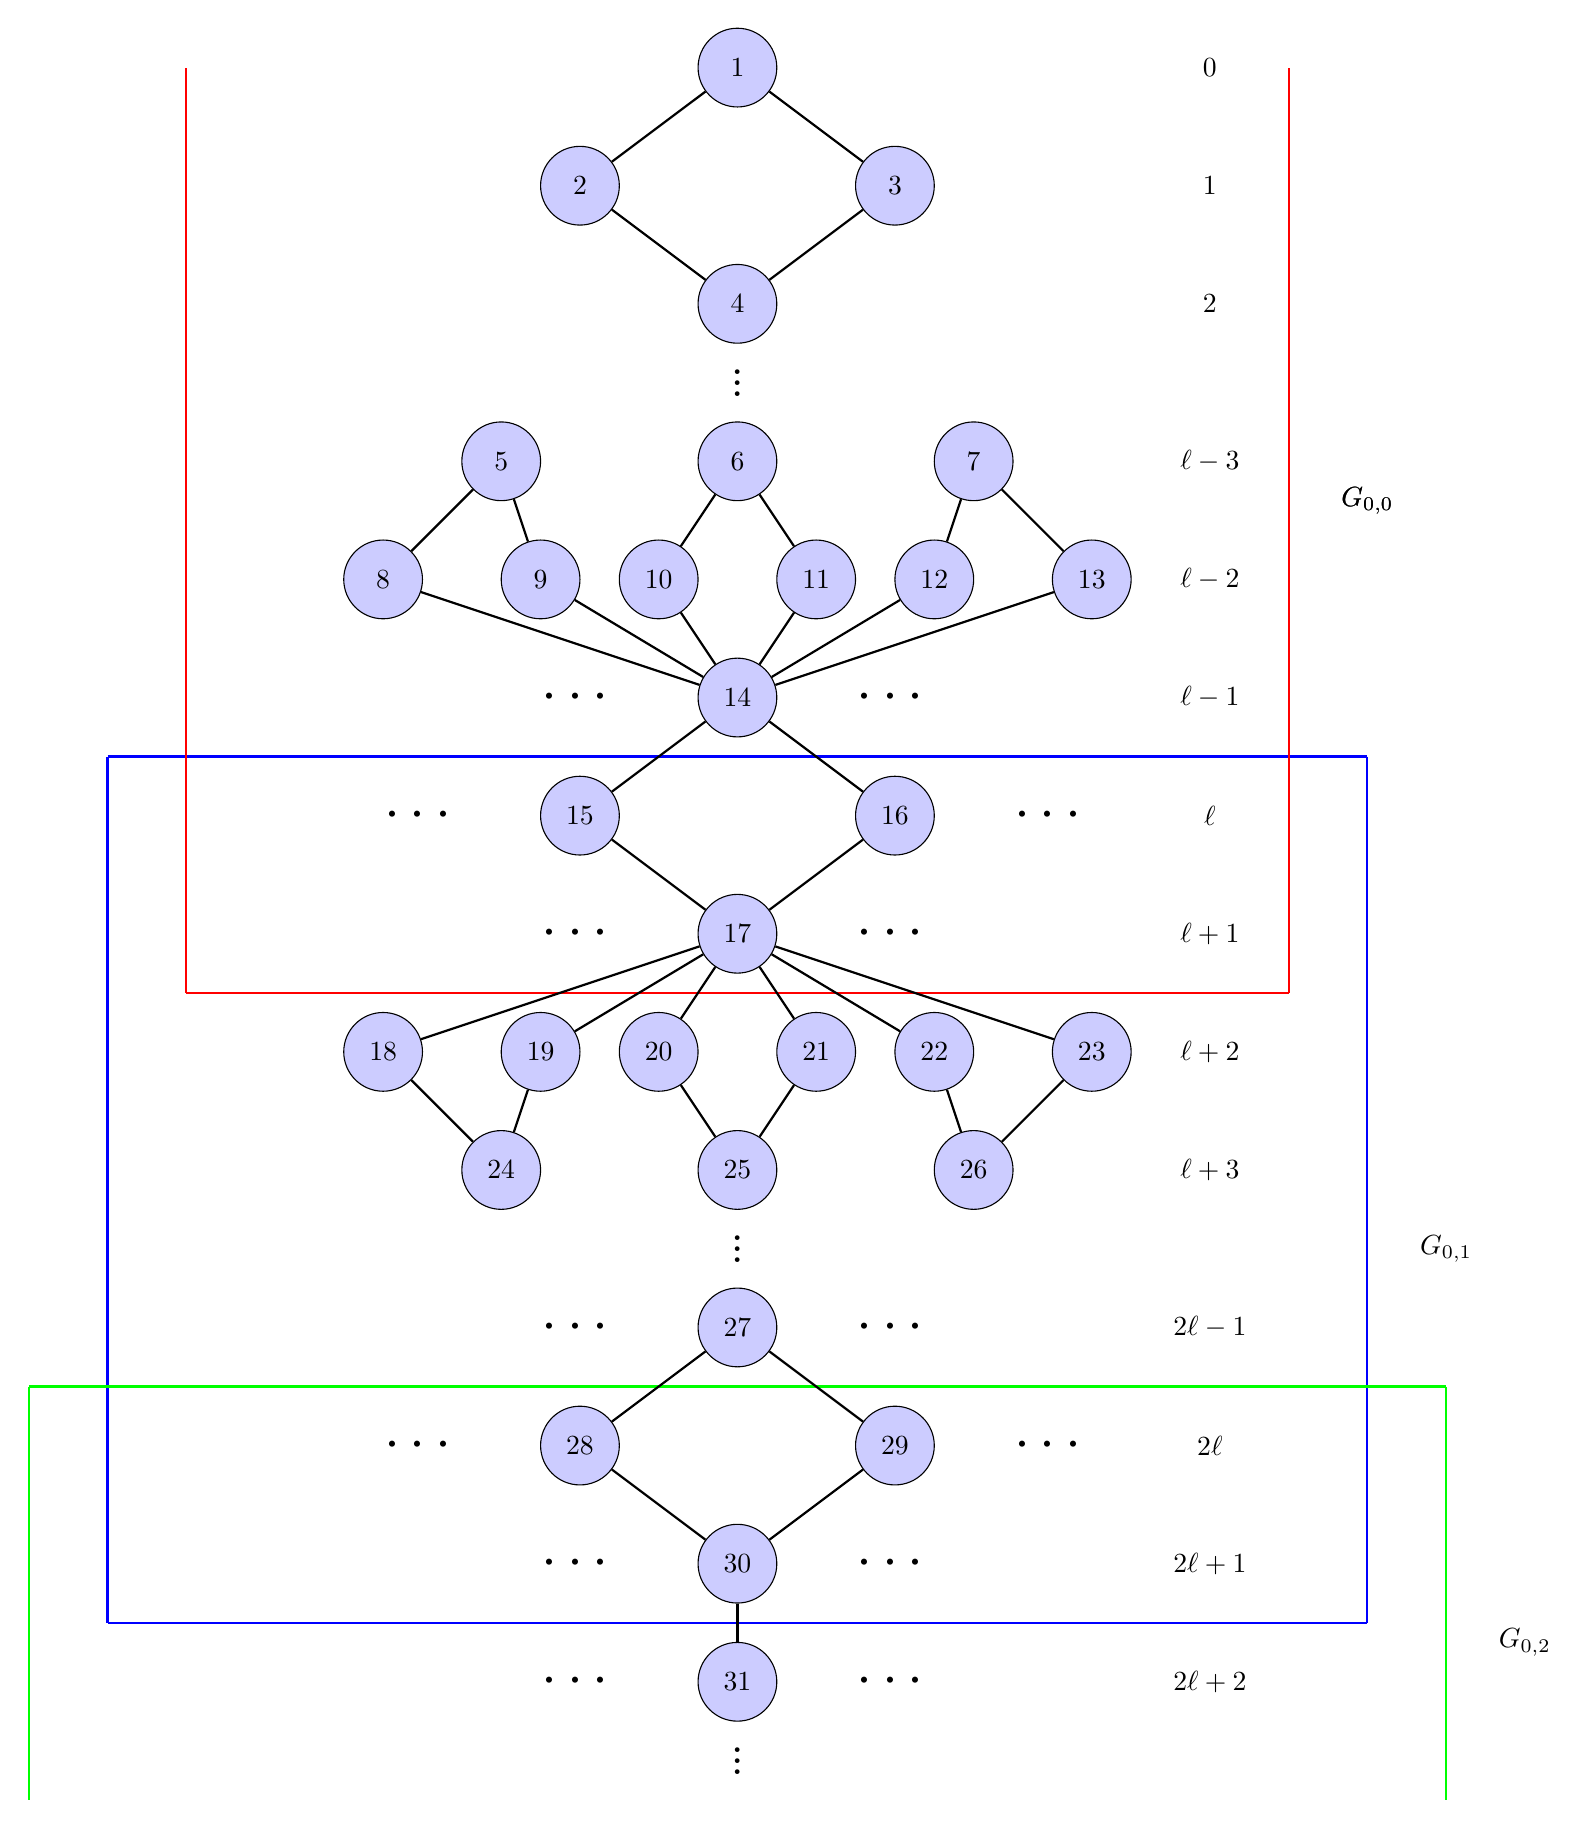
\begin{tikzpicture}
        % Level 0 (Root node)
        \node[circle, draw, fill=blue!20, minimum size=10mm] (1) at (0, 0) {1};

        % Level 1
        \node[circle, draw, fill=blue!20, minimum size=10mm] (2) at (-2, -1.5) {2};
        \node[circle, draw, fill=blue!20, minimum size=10mm] (3) at (2, -1.5) {3};

        % Level 2
        \node[circle, draw, fill=blue!20, minimum size=10mm] (4) at (0, -3) {4};

        % Dotted vertical line indicating further levels
        \node[draw=none] at (0, -3.9) { \huge $\vdots$ };

        % Level l-3
        \node[circle, draw, fill=blue!20, minimum size=10mm] (5) at (-3, -5){5};
        \node[circle, draw, fill=blue!20, minimum size=10mm] (6) at (0, -5) {6};
        \node[circle, draw, fill=blue!20, minimum size=10mm] (7) at (3, -5) {7};

        % Level l-2
        \node[circle, draw, fill=blue!20, minimum size=10mm] (8) at (-4.5, -6.5){8};
        \node[circle, draw, fill=blue!20, minimum size=10mm] (9) at (-2.5, -6.5) {9};
        \node[circle, draw, fill=blue!20, minimum size=10mm] (10) at (-1, -6.5) {10};
        \node[circle, draw, fill=blue!20, minimum size=10mm] (11) at (1, -6.5) {11};
        \node[circle, draw, fill=blue!20, minimum size=10mm] (12) at (2.5, -6.5) {12};
        \node[circle, draw, fill=blue!20, minimum size=10mm] (13) at (4.5, -6.5) {13};
        
        % Level l-1
        \node[circle, draw, fill=blue!20, minimum size=10mm] (14) at (0, -8){14};

        \node[draw=none] at (2, -8) {\huge $\cdots$};
        \node[draw=none] at (-2, -8) {\huge $\cdots$};

        % Vertical line between levels l-1 and l
        \draw[thick, blue] (-8, -8.75) -- (8, -8.75);
        \draw[thick, blue] (-8, -8.75) -- (-8, -19.75);
        \draw[thick, blue] (8, -8.75) -- (8, -19.75);
        \draw[thick, blue] (-8, -19.75) -- (8, -19.75);
        \node[draw=none] at (9, -15) {$G_{0, 1}$};

        % Level l
        \node[circle, draw, fill=blue!20, minimum size=10mm] (15) at (-2, -9.5){15};
        \node[circle, draw, fill=blue!20, minimum size=10mm] (16) at (2, -9.5){16};

        \node[draw=none] at (4, -9.5) {\huge $\cdots$};
        \node[draw=none] at (-4, -9.5) {\huge $\cdots$};

        % Level l+1
        \node[circle, draw, fill=blue!20, minimum size=10mm] (17) at (0, -11){17};
        
        % Vertical line between levels l+1 and l+2
        \draw[thick, red] (-7, -11.75) -- (7, -11.75);
        \draw[thick, red] (-7, -11.75) -- (-7, 0);
        \draw[thick, red] (7, -11.75) -- (7, 0);
        \node[draw=none] at (8, -5.5) {$G_{0, 0}$};

        % Horizontal dots on level l+1
        \node[draw=none] at (2, -11) {\huge $\cdots$};
        \node[draw=none] at (-2, -11) {\huge $\cdots$};

        % Level l+2
        \node[circle, draw, fill=blue!20, minimum size=10mm] (18) at (-4.5, -12.5){18};
        \node[circle, draw, fill=blue!20, minimum size=10mm] (19) at (-2.5, -12.5) {19};
        \node[circle, draw, fill=blue!20, minimum size=10mm] (20) at (-1, -12.5) {20};
        \node[circle, draw, fill=blue!20, minimum size=10mm] (21) at (1, -12.5) {21};
        \node[circle, draw, fill=blue!20, minimum size=10mm] (22) at (2.5, -12.5) {22};
        \node[circle, draw, fill=blue!20, minimum size=10mm] (23) at (4.5, -12.5) {23};
        
        % Level l+3
        \node[circle, draw, fill=blue!20, minimum size=10mm] (24) at (-3, -14){24};
        \node[circle, draw, fill=blue!20, minimum size=10mm] (25) at (0, -14) {25};
        \node[circle, draw, fill=blue!20, minimum size=10mm] (26) at (3, -14) {26};

        % Dotted vertical line indicating further levels
        \node[draw=none] at (0, -14.9) { \huge $\vdots$ };

        % Level 2l - 1
        \node[circle, draw, fill=blue!20, minimum size=10mm] (27) at (0, -16) {27};

        \node[draw=none] at (2, -16) {\huge $\cdots$};
        \node[draw=none] at (-2, -16) {\huge $\cdots$};

        % Vertical line between levels l+1 and l+2
        \draw[thick, green] (-9, -16.75) -- (9, -16.75);
        \draw[thick, green] (-9, -16.75) -- (-9, -22);
        \draw[thick, green] (9, -16.75) -- (9, -22);
        \node[draw=none] at (8, -5.5) {$G_{0, 0}$};

        % Level 2l
        \node[circle, draw, fill=blue!20, minimum size=10mm] (28) at (-2, -17.5) {28};
        \node[circle, draw, fill=blue!20, minimum size=10mm] (29) at (2, -17.5) {29};
        
        \node[draw=none] at (4, -17.5) {\huge $\cdots$};
        \node[draw=none] at (-4, -17.5) {\huge $\cdots$};

        % Level 2l+1
        \node[circle, draw, fill=blue!20, minimum size=10mm] (30) at (0, -19) {30};

        \node[draw=none] at (2, -19) {\huge $\cdots$};
        \node[draw=none] at (-2, -19) {\huge $\cdots$};

        % Level 2l+2
        \node[circle, draw, fill=blue!20, minimum size=10mm] (31) at (0, -20.5) {31};

        \node[draw=none] at (2, -20.5) {\huge $\cdots$};
        \node[draw=none] at (-2, -20.5) {\huge $\cdots$};

        % Dotted vertical line indicating further levels
        \node[draw=none] at (0, -21.4) { \huge $\vdots$ };

        \node[draw=none] at (10, -20) {$G_{0, 2}$};


        % Draw edges for BFS with renumbered vertices
        \foreach \I/\j in {1/2, 1/3, 2/4, 3/4, 5/8, 5/9, 8/14, 9/14, 6/10, 6/11, 10/14, 11/14,
        7/12, 7/13, 12/14, 13/14, 14/15, 14/16, 15/17, 16/17, 17/18, 17/19, 17/20, 17/21, 17/22, 17/23,
        18/24, 19/24, 20/25, 21/25, 22/26, 23/26, 27/28, 27/29, 28/30, 29/30, 30/31}
            \draw[thick] (\I) -- (\j);

        \node[draw=none] at (6, 0) {0};
        \node[draw=none] at (6, -1.5) {1};
        \node[draw=none] at (6, -3) {2};

        \node[draw=none] at (6, -5) {$\ell-3$};
        \node[draw=none] at (6, -6.5) {$\ell-2$};
        \node[draw=none] at (6, -8) {$\ell-1$};
        \node[draw=none] at (6, -9.5) {$\ell$};
        \node[draw=none] at (6, -11) {$\ell+1$};
        \node[draw=none] at (6, -12.5) {$\ell+2$};
        \node[draw=none] at (6, -14) {$\ell+3$};

        \node[draw=none] at (6, -16) {$2\ell-1$};
        \node[draw=none] at (6, -17.5) {$2\ell$};
        \node[draw=none] at (6, -19) {$2\ell+1$};

        \node[draw=none] at (6, -20.5) {$2\ell+2$};

    \end{tikzpicture}
\end{center}

\noindent Let $G$ look like the graph we sketched on the previous page. The vertical dots help us 
clarify the levels while the horizontal signify that there may be other vertices of interest. However, 
there are vertices we would like to inspect, specifically vertices with labels $14$ and $17$. Let 
$v_{14}, v_{17} \in F$. What follows is that $v_{14}, v_{17} \in F_{0, 0}$. The cycles that give us
reason to claim that $v_{14} \in F$ are all within $G_{0, 0}$. Therefore, it holds that
Algorithm~\ref{alg:ufvsbcl} will have $v_{14} \in S_{0, 0}$. However, the same does not hold for 
$v_{17}$, the cycles that it is a part of are in $G_{0, 1}$ and thus $v_{17} \notin S_{0, 0}$, while 
$v_{17} \in F_{0, 0}$. Thus we will be counting $v_{17}$ twice when we are combining the solutions
$F_{i, j}$, once in $F_{0, 0}$ and once in $F_{0, 1}$. This is what enables us to obtain an upper bound 
for $S$.
\section{Exact algorithm for FVS-4CL using MSOL}
\label{subsection:exact-alg}

In this section we are looking for an algorithm that finds exact solutions to the 
FVS-4CL problem in each subgraph. For each subgraph we assume that the treewidth is bounded. 

We take a logical approach that was introduced by Courcelle~\cite{courcelle1990monadic}. 
He shows that graph properties, that can be stated in monadic second-order logic (MSOL), can be solved in 
linear time for graphs of bounded treewidth. In the following two subsections we briefly explain MSOL and 
then apply it to our problem. We follow a survey on the matter in Satzinger \cite{satzinger2014tree}. 

\subsection{MSOL - a language for graph problems}

 We want to introduce a language that translates graph problems to formulas, therefore reducing 
the problem to a satisfiability problem. Consequently, our goal is to find a formula $\Phi$ with the 
property: 

\[\text{The problem $\Pi$ is solvable for a graph $G$ \textit{iff} $G \models \Phi$, i. e. the formula 
$\Phi$ is satisfied by the graph $G$.}\]

Problem $\Pi$ is solvable in polynomial (in this case linear) time for graphs of treewidth at 
most $k$.

Monadic second-order logic is an extension of first-order logic. Additionally to having 
object variables $x, y \dots$, logical connectives $\lnot, \land, \lor, \lnot,
\rightarrow, \longleftrightarrow$ and quantifiers for object variables $\forall x, 
\exists x$, MSOL considers sets of object variables $X, Y \dots$, and relation to them 
via $\in$.

Whenever graph problems are involved, typically we express solution through 
vertices and edges. Additionally, as we mentioned, we can construct sets of vertices 
and edges. Therefore we have the following machinery:

\begin{enumerate}[label=\textbf{•}]
    \item Object variables: \textit{vertices}: $v_1, v_2, \dots$ and \textit{edges}: $e_1, e_2, \dots$. 
    \item Set variables: sets of vertices $V_1, V_2, \dots$ and sets of edges $E_1, E_2, \dots$.
    \item Binary relation $\in : \{\text{object variable}\} \times \{\text{set variable}\} \to \{0, 1\}$. Therefore 
    $v \in V$ \textit{iff} $v$ is an element of the corresponding set $V$.
    \item The $Adj(e, v_i, v_j)$ relation. It detects whether edge $e$ is an edge from vertex $v_i$ to 
    vertex $v_j$ where $v_i \neq v_j$.
\end{enumerate}

 With this machinery, one obtains a first-order language suitable for expressing relations in a graph. 
To extend this to a traditional second-order logic language, one must add quantifications over set 
variables. 

\begin{enumerate}[label=\textbf{•}]
    \item Quantification over set variables: $\forall V_i, \forall E_i$ and $\exists V_i, \exists E_i$.
\end{enumerate}

\subsection{Exact algorithm for FVS-4CL using MSOL}

Courcelle's work was extended to extended monadic second-order logic 
\cite{arnborg1991easy,borie1991deterministic,courcelle1993monadic}. These extensions allow to optimize 
over the size and weight of a free set variable.

\begin{equation}
    \label{courcelle:unweighted}
    \begin{aligned}
        \min_{F \subseteq V} & \ |F| \\
        & \land \forall v \forall u \forall w \forall z \\
        & v \in (V \backslash F) \land u \in (V \backslash F) \land w \in (V \backslash F) \land z \in (V \backslash F) \\
        & \land v \neq w \land u \neq z \\
        & \land \neg ((v, u) \in E \land (u, w) \in E \land (w, z) \in E \land (v, z) \in E)
    \end{aligned}
\end{equation}

The minimum weight FVS-4CL can be expressed as:

\begin{equation}
    \label{courcelle:weighted}
    \begin{aligned}
        \min_{F \subseteq V} & \ w(F): \\
        & \forall v \forall u \forall w \forall z \\
        & v \in (V \backslash F) \land u \in (V \backslash F) \land w \in (V \backslash F) \land z \in (V \backslash F) \\
        & \land v \neq w \land u \neq z \\
        & \land \neg((v, u) \in E \land (u, w) \in E \land (w, z) \in E \land (v, z) \in E)
    \end{aligned}
\end{equation}


\subsection{Exact algorithm for weighted FVS-BCL using MSOL}

 The minimum weight FVS-$\rho$CL can be expressed as:

\begin{equation}
    \label{courcelle:rho}
    \begin{aligned}
        \min_{F \subseteq V} & \ w(F) : \\
        & \land \forall v_1 \forall v_2 \dots \forall v_{\rho} \\
        & v_1 \in (V \backslash F) \land v_2 \in (V \backslash F) \dots \land v_{\rho} \in (V \backslash F) \\
        & \land (v_1 \neq v_2 \land v_1 \neq v_3 \land \dots \land v_1 \neq v_{\rho}) \\ 
        & \land (v_2 \neq v_1 \land v_2 \neq v_3 \land \dots \land v_2 \neq v_{\rho}) \\
        & \dots \\
        & \land (v_{\rho} \neq v_1 \land v_{\rho} \neq v_2 \land \dots \land v_{\rho} \neq v_{\rho-1}) \\
        & \land \neg((v_1, v_2) \in E \land (v_2, v_3) \in E \land \dots \land (v_{\rho-1},v_{\rho}) \in E \land (v_{\rho}, v_1) \in E)
    \end{aligned}
\end{equation}


\refstepcounter{definition}
\begin{mydefinition}[Courcelle's theorem \cite{courcelle1990monadic}]{Theorem}
    \label{theorem:courcelle}

    Assume that $\phi$ is a MSOL formula and $G$ is an n-vertex graph, and there is an evaluation 
    of all of the free variables of $\phi$. Suppose, that a tree decomposition of $G$ of width $t$ 
    is provided. Then there exists an algorithm that verifies that $\phi$ is satisfied 
    in $G$ in time $f(||\phi||, t) \cdot n$, for some computable function $f$. 
    
\end{mydefinition}

\refstepcounter{definition}
\begin{mydefinition}[MSOL Solvability of FVS-$\rho$CL on Bounded-Treewidth Graphs]{Corollary}
    \label{cor:msol-fvs-rho}
    Let $\rho\ge 3$ be a constant, and let $G=(V,E)$ be an undirected graph of treewidth at 
    most $\tw$, equipped with a vertex-weight function $w:V\to\mathbb{N}$.  Then the 
    minimum-weight feedback-vertex-set that breaks all $\rho$-cycles in $G$ 
    (i.e.\ solves FVS-$\rho$CL) can be computed in time
    \[
        f(\rho, \tw) \cdot n^{\mathcal{O}(1)},
    \]
    where $f$ is some computable function depending only on $\rho$ and $\tw$. 
\end{mydefinition}
  

\subsection{Exact algorithm for FVS-4CL using dynamic programming}

\label{alg:dp}

In order to find an algorithm that solves FVS-4CL, one has to define the following notions. 
For a more thorough explanation of those concepts, see Bodlaender~\cite[Section 4.]{bodlaender1997treewidth}.

\begin{enumerate}
    \item Define the notion of a \textit{solution}. In our case for the FVS-4CL problem, the solution for a graph 
    $G$ is a set $F$, such that $G - F$ does not contain any cycles of length four.

    \item Define the notion of a \textit{partial solution}.
    For the subgraph $G_i = (V_i, E_i)$, partial solutions $F_i$ are restrictions of solutions 
    given by the subsets $F_i \subseteq V_i$. 
    
    \item Define the notion of \textit{extension of a partial solution}. A solution $F$ is an extension 
    of a partial solution $F_i$ for $G_i$ if $F \cap V_i = F_i$.

    \item Define the notion of a \textit{characteristic} of a partial solution. 
    For the set $X_i$ the vertices are partitioned twofold.

    \begin{enumerate}
        \item The class $I \subseteq X_i$ corresponds to all vertices that are in the partial solution 
        for the current node $X_i$.
        \item The class $\mathcal{F} \subseteq X_i \times X_i$ is comprised of all of the pairs of 
        vertices $v,u \in X_i: 
        (v, u) \in \Phi$ if they have a common neighbour $w \in V_i \backslash X_i$, such that 
        $w \notin F_i$.
    \end{enumerate}
    
    \[ch(G_i, F_i) = (\{v \in X_i: v \in F_i\}, 
    \{(v, u) \in X_i \times X_i: \exists w \in V_i \backslash X_i, 
    (v, w) \in E_i, (u, w) \in E_i, w \notin F_i\})\]

    The valuation of a characteristic $ch(G_i, F_i)$ is a table $c[i, I, \mathcal{F}]$.
    It represents the minimum weight 
    of a partial solution $F_i$ in $G_i$ and $c[i, I, \mathcal{F}] \in \mathbb{N} \cup \{\infty\}$.
    The table keeps the value of infinity if no such set exists.

    \[c[i, I, \mathcal{F}] = \min\{w(W) : W \text{ is a FVS-4CL of } G_i \land W \cap X_i = I\}\] 

    \item Define the notion of a \textit{full set of characteristics}.

    The full set for a node $X_i$ is a valuation for each characteristic $I \in \{0, 1\}^{|X_i|}$ 
    and $\mathcal{F} \in \{0, 1\}^{X_i \times X_i}$. Since there are at most $\tw+1$ elements, 
    there are at most $2^{(\tw+1)} \cdot 2^{\binom{\tw+1}{2}}$ entries. That yields a storage 
    capacity of $2^{\binom{\tw+1}{2} + (\tw+1)} = 2^{\mathcal{O}(\tw^2)}$. 

\end{enumerate}

\textbf{Leaf node:}

For a leaf node $i$, we have that $X_i = \emptyset$. Hence 

\[c[i, \emptyset, \emptyset] = 0\]

\textbf{Introduce node:}

Let $i$ be an introduce node with child node $j$. We have that $X_i = X_j \cup \{v\}$ for some 
vertex $v \notin X_j$. There are two possible values.
\[
\begin{aligned}
    c[i, I \cup \{v\}, \mathcal{F}] &= w(v) + c[j, I, \mathcal{F}] \\
    c[i, I, \mathcal{F}] &= 
    \begin{cases}
        \infty, & \text{if } \exists u, w \in X_i: (u, w) \in \mathcal{F}, u \notin I, w \notin I, (v, u) \in E_i, (v, w) \in E_i \\
        c[j, I, \mathcal{F}], & \text{otherwise}
    \end{cases}
\end{aligned}
\]

\textbf{Forget node:}

Let $i$ be a forget node with child node $j$. We have that $X_i = X_j \backslash \{v\}$ for 
some vertex $v \in X_j$.

\[c[i, I, \mathcal{F}] = \min(c[j, I \cup \{v\}, \mathcal{F}],
c[j, I, \mathcal{F} \cup \{(u, w): (v,u) \in E_i, (v, w) \in E_i\}])\]

\textbf{Join node:}

Let $i$ be a join node with children $j_1$ and $j_2$. Recall that $X_i = X_{j_1} = X_{j_2}$. 
Let $\mathcal{F}_1$ and $\mathcal{F}_2$ be the $\mathcal{F}$ set values of $X_{j_1}$ and $X_{j_2}$ respectively.

\[
\begin{aligned}
    c[i, I, \mathcal{F}_1 \cup \mathcal{F}_2] =
    \begin{cases}
        \infty, & \text{if } \exists u, w \in X_i : (u, w) \in \mathcal{F}_1, \\
                & \quad (u, w) \in \mathcal{F}_2, u \notin I, w \notin I \\
        c[j_1, I, \mathcal{F}_1] + c[j_2, I, \mathcal{F}_2] - w(I), & \text{otherwise}
    \end{cases}
\end{aligned}
\]


\section{m-stitching and $\Pi$-m-stitching}

This section introduces key concepts that facilitate the construction of certified algorithms. 
It begins with the definitions of \textit{m-stitching} and \textit{$\Pi$-m-stitching}, 
followed by a presentation of the main theorem from 
Bumpus et al.~\cite{bumpus_et_al:LIPIcs.SWAT.2024.19}. 
These concepts and the theorem will be used for constructing certified algorithms 
in the following section. 
Unless stated otherwise, $\Pi$ is assumed to be a vertex-minimization problem.
We refer to the literature in \cite{bumpus_et_al:LIPIcs.SWAT.2024.19, venne2022designing}.

\subsection{FVS-4CL and 2-stitching}

The restriction we imposed on the Feedback Vertex Set problem enables us to look 
for optimal solutions in a local space. This is what m-stitching and $\Pi$-m-stitching
hint at. Here, the the variable $m$ is a positive integer that depends on the vertex optimization 
problem $\Pi$. In our case this is tied to the $\rho$ argument, i. e. the length of 
the cycles one is trying to break. 

To introduce $\Pi$-m-stitching, it is essential to first understand m-stitching 
and m-stitchable problems. In the stitching operation, two solutions $S_1$ and $S_2$ 
are given for a vertex optimization problem, along with an induced subgraph $J$ of $G$. 
Intuitively, the idea is to take the portion of $S_1$ that lies outside of $J$ 
and stitch onto it a suitable part of $S_2$ within the subgraph $J$.

The formal definition is as follows:

\refstepcounter{definition}
\begin{mydefinition}[m-stitching]{Def.}
    \label{m-stitch}

    Assume $m \geq 0$ is an integer, $J$ is an induced subgraph of $G$, and 
    $S_1, S_2 \subseteq V(G)$. Then we define the \textit{m-stitch} of $S_2$ onto $S_1$ along 
    $J$ as the set:

    \[S_3 := (S_1 \backslash J) \cup (S_2 \cap N^{m}_{G} \left[J\right]).\]

\end{mydefinition}

\begin{figure}[H]
    \centering
    \begin{minipage}{0.50\textwidth}
        \centering
        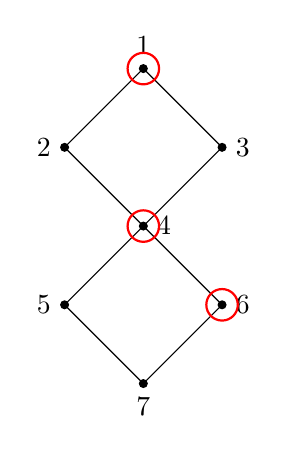
\begin{tikzpicture}
            % Define nodes
            \node[draw, circle, fill=black, scale=0.3, label=above:1] (1) at (0,2) {};
            \node[draw, circle, fill=black, scale=0.3, label=left:2] (2) at (-1,1) {};
            \node[draw, circle, fill=black, scale=0.3, label=right:3] (3) at (1,1) {};
            \node[draw, circle, fill=black, scale=0.3, label=right:4] (4) at (0,0) {};
            \node[draw, circle, fill=black, scale=0.3, label=left:5] (5) at (-1,-1) {};
            \node[draw, circle, fill=black, scale=0.3, label=right:6] (6) at (1,-1) {};
            \node[draw, circle, fill=black, scale=0.3, label=below:7] (7) at (0,-2) {};

            % Draw edges
            \draw (1) -- (2);
            \draw (1) -- (3);
            \draw (2) -- (4);
            \draw (3) -- (4);
            \draw (4) -- (5);
            \draw (4) -- (6);
            \draw (5) -- (7);
            \draw (6) -- (7);


            \draw[red, thick] (1) circle(0.2);
            \draw[red, thick] (4) circle(0.2);
            \draw[red, thick] (6) circle(0.2);

        \end{tikzpicture}
        \caption{Vertex set $S_1$}
    \end{minipage}
    \hfill
    \begin{minipage}{0.49\textwidth}
        \centering
        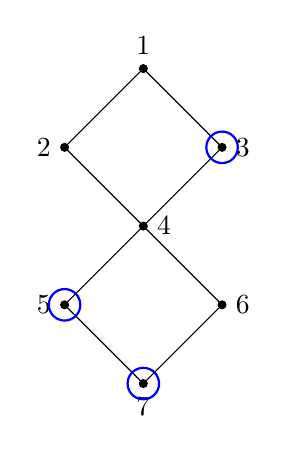
\begin{tikzpicture}
            % Define nodes
            \node[draw, circle, fill=black, scale=0.3, label=above:1] (1) at (0,2) {};
            \node[draw, circle, fill=black, scale=0.3, label=left:2] (2) at (-1,1) {};
            \node[draw, circle, fill=black, scale=0.3, label=right:3] (3) at (1,1) {};
            \node[draw, circle, fill=black, scale=0.3, label=right:4] (4) at (0,0) {};
            \node[draw, circle, fill=black, scale=0.3, label=left:5] (5) at (-1,-1) {};
            \node[draw, circle, fill=black, scale=0.3, label=right:6] (6) at (1,-1) {};
            \node[draw, circle, fill=black, scale=0.3, label=below:7] (7) at (0,-2) {};

            % Draw edges
            \draw (1) -- (2);
            \draw (1) -- (3);
            \draw (2) -- (4);
            \draw (3) -- (4);
            \draw (4) -- (5);
            \draw (4) -- (6);
            \draw (5) -- (7);
            \draw (6) -- (7);

            \draw[blue, thick] (3) circle(0.2);
            \draw[blue, thick] (5) circle(0.2);
            \draw[blue, thick] (7) circle(0.2);

        \end{tikzpicture}
        \caption{Vertex set $S_2$}
    \end{minipage}
\end{figure}

 In the following we show the subgraph $J$ we have chosen and the 2-neighbourhood 
of the subgraph.

 Also, in Fig.~\ref{fig:remove_s1} we show the first step of the m-stitch operation, namely 
removing the vertices of $J$ from the set $S_1$.

\begin{figure}[H]
    \centering
    \begin{minipage}{0.50\textwidth}
        \centering
        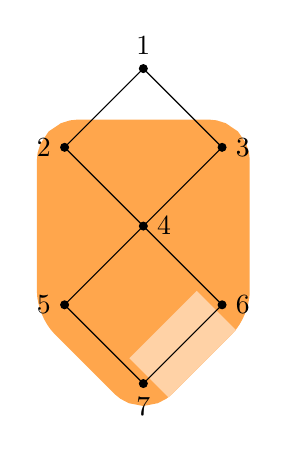
\begin{tikzpicture}
            % Define nodes
            \node[draw, circle, fill=black, scale=0.3, label=above:1] (1) at (0,2) {};
            \node[draw, circle, fill=black, scale=0.3, label=left:2] (2) at (-1,1) {};
            \node[draw, circle, fill=black, scale=0.3, label=right:3] (3) at (1,1) {};
            \node[draw, circle, fill=black, scale=0.3, label=right:4] (4) at (0,0) {};
            \node[draw, circle, fill=black, scale=0.3, label=left:5] (5) at (-1,-1) {};
            \node[draw, circle, fill=black, scale=0.3, label=right:6] (6) at (1,-1) {};
            \node[draw, circle, fill=black, scale=0.3, label=below:7] (7) at (0,-2) {};

            % Draw edges
            \draw (1) -- (2);
            \draw (1) -- (3);
            \draw (2) -- (4);
            \draw (3) -- (4);
            \draw (4) -- (5);
            \draw (4) -- (6);
            \draw (5) -- (7);
            \draw (6) -- (7);

            \begin{scope}[on background layer]
                \filldraw[orange!70,line width=20pt,rounded corners=5pt] (2.center) -- (3.center) -- (6.center) -- (7.center) -- (5.center) -- cycle;
            \end{scope}

            \begin{scope}[on background layer]   
                \filldraw[orange!35,line width=20pt,rounded corners=5pt] (6.center) --  (7.center) -- cycle;
            \end{scope}

        \end{tikzpicture}
        \caption{Subgraph $J$ of $G$ in light orange and $N^{2}_{G}\left[J\right]$ in darker orange}
    \end{minipage}
    \hfill
    \begin{minipage}{0.49\textwidth}
        \centering
        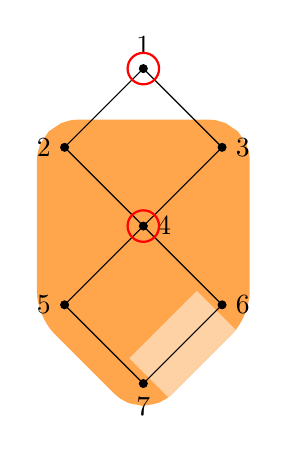
\begin{tikzpicture}
            % Define nodes
            \node[draw, circle, fill=black, scale=0.3, label=above:1] (1) at (0,2) {};
            \node[draw, circle, fill=black, scale=0.3, label=left:2] (2) at (-1,1) {};
            \node[draw, circle, fill=black, scale=0.3, label=right:3] (3) at (1,1) {};
            \node[draw, circle, fill=black, scale=0.3, label=right:4] (4) at (0,0) {};
            \node[draw, circle, fill=black, scale=0.3, label=left:5] (5) at (-1,-1) {};
            \node[draw, circle, fill=black, scale=0.3, label=right:6] (6) at (1,-1) {};
            \node[draw, circle, fill=black, scale=0.3, label=below:7] (7) at (0,-2) {};

            % Draw edges
            \draw (1) -- (2);
            \draw (1) -- (3);
            \draw (2) -- (4);
            \draw (3) -- (4);
            \draw (4) -- (5);
            \draw (4) -- (6);
            \draw (5) -- (7);
            \draw (6) -- (7);

            \begin{scope}[on background layer]   
                \filldraw[orange!70,line width=20pt,rounded corners=5pt] (2.center) -- (3.center) -- (6.center) -- (7.center) -- (5.center) -- cycle;
            \end{scope}

            \begin{scope}[on background layer]   
                \filldraw[orange!35,line width=20pt,rounded corners=5pt] (6.center) --  (7.center) -- cycle;
            \end{scope}

            \draw[red, thick] (1) circle(0.2);
            \draw[red, thick] (4) circle(0.2);

        \end{tikzpicture}
        \caption{Remove $J$ from $S_1$}
        \label{fig:remove_s1}
    \end{minipage}
\end{figure}

 What follows is the second step in obtaining set $S_3$ in Fig.~\ref{fig:second_step} and the 
stitched set in Fig.~\ref{fig:stitched_set}.

\begin{figure}[H]
    \centering
    \begin{minipage}{0.50\textwidth}
        \centering
        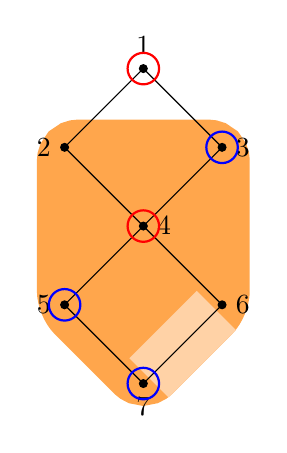
\begin{tikzpicture}
            % Define nodes
            \node[draw, circle, fill=black, scale=0.3, label=above:1] (1) at (0,2) {};
            \node[draw, circle, fill=black, scale=0.3, label=left:2] (2) at (-1,1) {};
            \node[draw, circle, fill=black, scale=0.3, label=right:3] (3) at (1,1) {};
            \node[draw, circle, fill=black, scale=0.3, label=right:4] (4) at (0,0) {};
            \node[draw, circle, fill=black, scale=0.3, label=left:5] (5) at (-1,-1) {};
            \node[draw, circle, fill=black, scale=0.3, label=right:6] (6) at (1,-1) {};
            \node[draw, circle, fill=black, scale=0.3, label=below:7] (7) at (0,-2) {};

            % Draw edges
            \draw (1) -- (2);
            \draw (1) -- (3);
            \draw (2) -- (4);
            \draw (3) -- (4);
            \draw (4) -- (5);
            \draw (4) -- (6);
            \draw (5) -- (7);
            \draw (6) -- (7);

            \begin{scope}[on background layer]   
                \filldraw[orange!70,line width=20pt,rounded corners=5pt] (2.center) -- (3.center) -- (6.center) -- (7.center) -- (5.center) -- cycle;
            \end{scope}

            \begin{scope}[on background layer]   
                \filldraw[orange!35,line width=20pt,rounded corners=5pt] (6.center) --  (7.center) -- cycle;
            \end{scope}

            \draw[red, thick] (1) circle(0.2);
            \draw[red, thick] (4) circle(0.2);

            \draw[blue, thick] (3) circle(0.2);
            \draw[blue, thick] (5) circle(0.2);
            \draw[blue, thick] (7) circle(0.2);


        \end{tikzpicture}
        \caption{Add $S_2 \cap N^{2}_{G} \left[J\right]$}
        \label{fig:second_step}
    \end{minipage}
    \hfill
    \begin{minipage}{0.49\textwidth}
        \centering
        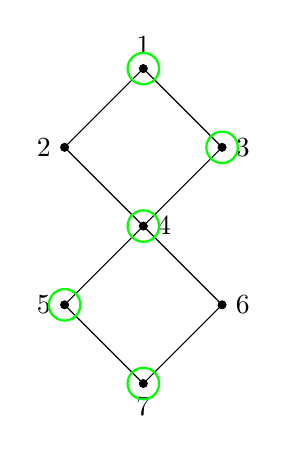
\begin{tikzpicture}
            % Define nodes
            \node[draw, circle, fill=black, scale=0.3, label=above:1] (1) at (0,2) {};
            \node[draw, circle, fill=black, scale=0.3, label=left:2] (2) at (-1,1) {};
            \node[draw, circle, fill=black, scale=0.3, label=right:3] (3) at (1,1) {};
            \node[draw, circle, fill=black, scale=0.3, label=right:4] (4) at (0,0) {};
            \node[draw, circle, fill=black, scale=0.3, label=left:5] (5) at (-1,-1) {};
            \node[draw, circle, fill=black, scale=0.3, label=right:6] (6) at (1,-1) {};
            \node[draw, circle, fill=black, scale=0.3, label=below:7] (7) at (0,-2) {};

            % Draw edges
            \draw (1) -- (2);
            \draw (1) -- (3);
            \draw (2) -- (4);
            \draw (3) -- (4);
            \draw (4) -- (5);
            \draw (4) -- (6);
            \draw (5) -- (7);
            \draw (6) -- (7);

            \draw[green, thick] (1) circle(0.2);
            \draw[green, thick] (3) circle(0.2);
            \draw[green, thick] (4) circle(0.2);
            \draw[green, thick] (5) circle(0.2);
            \draw[green, thick] (7) circle(0.2);

        \end{tikzpicture}
        \caption{Set $S_3$}
        \label{fig:stitched_set}
    \end{minipage}
\end{figure}

 A problem $\Pi$ is \textit{m-stitchable} if the set of feasible solutions are closed 
under the m-stitching operator. We hope that when we take the union in \ref{m-stitch} and arrive 
at the set $S_3$, this would too be a feasible solution.

\refstepcounter{definition}
\begin{mydefinition}[m-stitchable]{Def.}
    \label{m-stitchable}

    For an integer $m \geq 0$, induced subgraph $J$ and feasible solutions $S_1, S_2 \subseteq V(G)$ 
    of a vertex optimization problem $\Pi$ we have that the m-stitching of $S_2$ onto $S_1$ along 
    $J$, $S_3$ is a feasible solution to $\Pi$ on $G$.

    \[S_3 := (S_1 \backslash J) \cup (S_2 \cap N^{m}_{G} \left[J\right]).\]

\end{mydefinition}

 Now that we have a definition for problems $\Pi$ that are m-stitchable, we introduce 
$\Pi$-m-stitching as defined in \cite{bumpus_et_al:LIPIcs.SWAT.2024.19} and afterwards apply 
it to the current problem.

\refstepcounter{definition}
\begin{mydefinition}[$\Pi$-m-stitching]{Algorithm.}
    \label{alg:p-m-stitching}

    \textbf{Input:}
    an instance ($G, w : V(G) \to \mathbb{N}$) to an m-stitchable vertex optimization problem $\Pi$ 
    along with a solution $S_1$ and a vertex set $J \subseteq V(G)$.

    \textbf{Task:}
    find a feasible solution $S^{\prime}$ to $\Pi$ on $G$, such that for all other feasible solutions 
    $S^*$ it holds that $w(S^{\prime}) \leq w\left(S^{*} \oplus^{2}_{G,J} S_1\right)$.

\end{mydefinition}

 Before we proceed with the main theorem that we use to construct a certified algorithm 
we need one more definition.

\refstepcounter{definition}
\begin{mydefinition}[Guessable]{Def.}
    \label{guessable}

     A problem $\Pi$ is guessable if there is an algorithm that outputs a feasible solution 
    with no requirement for optimality in polynomial time.

\end{mydefinition}

 The following theorem is the main result in 
Bumpus et al.~\cite[Theorem 1.7]{bumpus_et_al:LIPIcs.SWAT.2024.19}.

\refstepcounter{definition}
\begin{mydefinition}[Main Theorem]{Theorem.}
    \label{theorem-main}

    Let $\mathbb{G}$ be a minor-closed graph class whose local tree-width is bounded above by a linear 
    function of the form $g : r \to \lambda \cdot r$ (fixed $\lambda \in \mathbb{R}$ and $r \in \mathbb{N}$).
    If $\Pi$ is a vertex-minimization problem and it holds that:

    \begin{enumerate}
        \item $\Pi$ is guessable.
        \item $\Pi$ is m-stitchable.
        \item There exists an algorithm $A_{\Pi}$ which solves $\Pi$-m-stitching in time $f(t) \cdot  |V(G)|^{\mathbb{O}(1)}$,
        where t = $\tw$($G\left[N^{m}_{G}(J)\right]$) and $f$ is a computable function;
    \end{enumerate}

    then, for each $\epsilon > 0$ there is a $(1 + \epsilon)$-certified algorithm for $\Pi$ that 
    runs in time $f(\lambda \cdot m / \epsilon) \cdot \left|V(G)\right| ^ {\mathbb{O}(1)}$ 
    on any input $(G, w : V(G) \to \mathbb{N})$ with $G \in \mathbb{G}$ and 
    polynomially-bounded weights.

\end{mydefinition}

 The proof of theorem \ref{theorem-main} is beyond the scope of this paper. In this section 
we only apply the three steps, mentioned to the FVS-BCL problem without generalizing to other 
vertex-minimization problems. 

 Firstly, we take a look at the guessable property.

\refstepcounter{definition}
\begin{mydefinition}[FVS-BCL is guessable]{Lemma}
    \label{lemma-guessable}

     For any planar graph $G$, the set $V(G)$ is a feasible solution to FVS-BCL.

\end{mydefinition}


\begin{proof}
    The graph $G - X$, where $X$ is the set of all vertices $V(G)$, is the empty graph, 
    therefore there are no 4-cycles left, after selecting that set.
\end{proof}

\refstepcounter{definition}
\begin{mydefinition}[FVS-BCL is 2-stitchable]{Lemma}
    \label{lemma-m-stitchable}

     Let $(G, w)$ be any instance to the FVS-4CL problem, $J \subseteq V(G)$, some subset
    of the vertices in the graph 
    and $S_1$ and $S_2$ any two feasible solutions to the problem in $G$. Then the set $S_3$:
    \[S_3 := (S_1 \backslash J) \cup (S_2 \cap N^{2}_{G} \left[J\right]).\]
    
    is a feasible solution to the problem.


\end{mydefinition}

\begin{proof}

Let the vertices $\{v_1,v_2,v_3,v_4\}$ form a 4-cycle.
We inspect the possible cases for the 4-cycle $v_1 v_2 v_3 v_4$. In order 
to prove \ref{lemma-m-stitchable} we have to prove that there exists a $v \in \{v_1, v_2, v_3, v_4\}$,
such that $v \in S_3$. 

\begin{enumerate}[label=\textbf{•}]
    \item $\exists v^{\prime} \in \{v_1,v_2,v_3,v_4\}$, such that $v^{\prime} \in J$. We argue in three steps.

    \begin{enumerate}
        \item Because $S_2$ is a feasible solution, then $\exists v'' \in \{v_1, v_2, v_3, v_4\}$,
        such that $v'' \in S_2$.
        \item Because there $\exists v' \in \{v_1,v_2,v_3,v_4\} \in J$, then it also holds
        that $\forall  v''' \in \{v_1,v_2,v_3,v_4\}, v''' \in N^{2}_{G}[J]$. From that and the previous 
        point it follows that $v'' \in S_2 \cap N^{2}_{G}[J]$.
        \item Finally, $S_2 \cap N^{2}_{G}[J] \subseteq S_3$, therefore $v'' \in S_3$.
    \end{enumerate}

    \item $\forall v' \in \{v_1,v_2,v_3,v_4\}$, it holds that $v' \notin J$.
    This case follows from the feasibility of $S_1$.

    \begin{enumerate}
        \item Because $S_1$ is a feasible solution, then $\exists v'' \in \{v_1,v_2,v_3,v_4\}$,
        such that $v'' \in S_1$.
        \item From $\forall v' \in \{v_1,v_2,v_3,v_4\} \notin J$ and the previous point, it follows 
        that $v'' \in S_1 \backslash J$.
        \item Because $S_1 \backslash J \subseteq S_3$, then $v'' \in S_3$.
    \end{enumerate}

\end{enumerate}

\end{proof}

 Now we describe an algorithm to find a feasible solution of minimum weight.

\begin{algorithm}[H]
    \caption{Stitch-FVS-4CL}
    \label{alg:stitch-fvs-4cl}
    \begin{algorithmic}[1]
    \REQUIRE Vertex-weighted planar graph $(G, w:V(G) \to \mathbb{N})$, a feasible solution $S_1$ on $G$
    and a vertex set $J \subseteq V(G)$
    .
    \ENSURE a feasible solution $S'$ on $G$, such that for all other feasible solutions $S^{*}$, 
    we have $w(S') \leq w(S^{*} \oplus^{2}_{G,J} S_1)$. 
    \STATE Let $H \leftarrow G[N^{2}_{G}[J] \backslash (S_1 \backslash J)]$. \label{state:construct-H}
    \STATE Let $S_2$ be the output of algorithm $A$ on input $(H, w)$. \label{state:opt-solution}
    \IF{ $w(S_2 \oplus^{2}_{G,J} S_1) < w(S_1)$ }
        \RETURN $S_2 \oplus^{2}_{G,J} S_1$
    \ELSE
        \RETURN $S_1$
    \ENDIF
    \end{algorithmic}
\end{algorithm}

The algorithm $A$ on line~\ref{alg:stitch-fvs-4cl} refers to calling 
Algorithm~\ref{courcelle:rho} that takes as input a graph that has bounded treewidth.


\refstepcounter{definition}
\begin{mydefinition}[FVS-4CL-2-stitching]{Lemma}
    \label{lemma-stictch-fvs-4cl}

    Let $A$ be an algorithm that solves FVS-4CL on any vertex-weighted instance $(G, w : V(G) \to \mathbb{N})$
    in time $f(t) \cdot |V(G)|^{O(1)}$ where $t$ is the treewidth of $G$. 
    Then Algorithm~\ref{alg:stitch-fvs-4cl} solves 
    FVS-4CL-2-stitching in time $f(\tw) \cdot n^{\mathcal{O}(1)}$ where 
    $\tw$ is the treewidth of $N^{2}_{G}[J]$. 
    In the end of the lemma we argue about the exact running time of the algorithm.
    
\end{mydefinition}

Note that it is not obvious that the set $S_2 \oplus^{2}_{G,J} S_1$ is a feasible solution in $G$ as $S_2$ is not 
necessarily a feasible solution in $G$. If the last was the case, then the feasibility of the 
$S_2 \oplus^{2}_{G,J} S_1$ would follow from Lemma~\ref{lemma-m-stitchable}. Therefore we first prove 
feasibility of $S_2 \oplus^{2}_{G,J} S_1$. Afterwards, we prove that it is of minimum weight.

\begin{proof}
    
We prove the feasibility of $S_2 \oplus^{2}_{G,J} S_1$ by case analysis on any four vertices
that form a 4-cycle. Remember that $S_2 \oplus^{2}_{G,J} S_1 = (S_1 \backslash J) \cup (S_2 \cap N^{2}_{G}[J])$.

\begin{enumerate}
    \item $\forall v' \in \{v_1,v_2,v_3,v_4\}: v' \in V(G) \backslash J$.

    Firstly, because of the feasibility of $S_1$, there $\exists v'' \in \{v_1,v_2,v_3,v_4\}: v'' \in S_1$.

    Secondly, $\forall v' \in \{v_1, v_2, v_3, v_4\}$, it holds that $v' \in V(G) \backslash J$.

    Finally from the first two conditions, using the property $A \backslash B = A \cap B^c$, 
    it holds that $v'' \in S_1 \backslash J$. From this
    and $S_1 \backslash J \subseteq S_2 \oplus^{2}_{G,J} S_1$, it follows that $S_2 \oplus^{2}_{G,J} S_1$ is feasible in $G$.

    In Fig.~\ref{fig:first-figure} we show (a part of) an example graph $G$ and the feasible solution 
    $S_1$ for it. In Fig.~\ref{fig:second-figure}, one can see that 4-cycles that do not have vertices 
    in $J$, are a part of $S_1 \backslash J \subseteq S_2 \oplus^{2}_{G,J} S_1$. 

    \begin{figure}[H]
        \centering
        \begin{minipage}{0.50\textwidth}
            \centering
            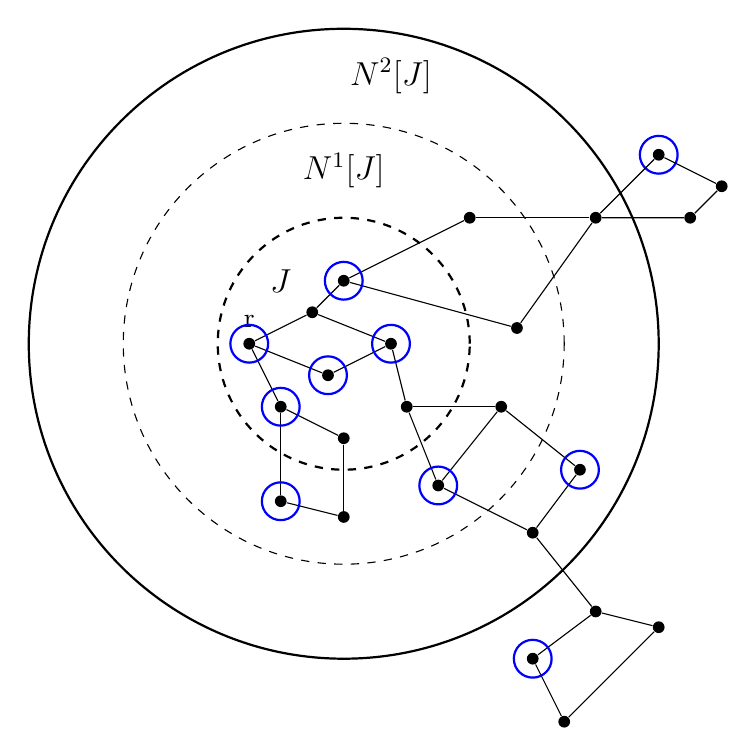
\begin{tikzpicture}[scale=0.8]
                %Draw J vertices
                \node[fill=black, circle, inner sep=1.5pt] (j01) at (0.75,0.5) {};
                \node[fill=black, circle, inner sep=1.5pt, label=above:r] (j02) at (-0.5,1) {};
                \node[fill=black, circle, inner sep=1.5pt] (j03) at (0.5,1.5) {};
                \node[fill=black, circle, inner sep=1.5pt] (j04) at (1.75,1) {};
        
                \node[fill=black, circle, inner sep=1.5pt] (j1) at (0,0) {};
                \node[fill=black, circle, inner sep=1.5pt] (j2) at (2,0) {};
                \node[fill=black, circle, inner sep=1.5pt] (j3) at (1,2) {};
                \node[fill=black, circle, inner sep=1.5pt] (j4) at (1,-0.5) {};
                
                % Draw N^1[J] vertices
        
                \node[fill=black, circle, inner sep=1.5pt] (n11) at (3.5,0) {};
                \node[fill=black, circle, inner sep=1.5pt] (n12) at (3.75,1.25) {};
                \node[fill=black, circle, inner sep=1.5pt] (n13) at (3,3) {};
                \node[fill=black, circle, inner sep=1.5pt] (n14) at (0,-1.5) {};
                \node[fill=black, circle, inner sep=1.5pt] (n15) at (1,-1.75) {};
                \node[fill=black, circle, inner sep=1.5pt] (n16) at (2.5,-1.25) {};
        
        
                % Draw N^2[J] vertices
                \node[fill=black, circle, inner sep=1.5pt] (n21) at (5, 3) {};
                \node[fill=black, circle, inner sep=1.5pt] (n22) at (4,-2) {};
                \node[fill=black, circle, inner sep=1.5pt] (n23) at (4.75,-1) {};
        
                % Draw vertices outside N^2[J]
                \node[fill=black, circle, inner sep=1.5pt] (n31) at (4, -4) {};
                \node[fill=black, circle, inner sep=1.5pt] (n32) at (5, -3.25) {};
                \node[fill=black, circle, inner sep=1.5pt] (n33) at (6, -3.5) {};
                \node[fill=black, circle, inner sep=1.5pt] (n34) at (4.5, -5) {};

                \node[fill=black, circle, inner sep=1.5pt] (new31) at (6, 4) {};
                \node[fill=black, circle, inner sep=1.5pt] (new32) at (6.5, 3) {};
                \node[fill=black, circle, inner sep=1.5pt] (new33) at (7, 3.5) {};
                
        
                % Draw edges inside J (induced subgraph)
                \draw (j01) -- (j02);
                \draw (j02) -- (j03);
                \draw (j03) -- (j04);
                \draw (j04) -- (j01);
        
                \draw (j4) -- (j1);

                \draw (j02) -- (j1);
                \draw (j04) -- (j2);
                \draw (j03) -- (j3);
                
                % Draw edges from J to N^1[J]
                \draw (j2) -- (n11);
                \draw (j2) -- (n16);
                \draw (j3) -- (n12);
                \draw (j1) -- (n14);
                \draw (j3) -- (n13);
                \draw (j4) -- (n15);
        
                % Draw edges inside N^1[J]
                \draw (n14) -- (n15);
                \draw (n16) -- (n11);
        
                % Draw edges between N^1[J] and N^2[J]
                \draw (n16) -- (n22);
                \draw (n11) -- (n23);
                \draw (n13) -- (n21);
                \draw (n12) -- (n21);
        
                % Draw edges between N^2[J] and N^2[J]
                \draw (n22) -- (n23);
        
                % Draw edges between N^2[J] and the other part of the graph
                \draw (n22) -- (n32);
        
                % Draw edges between the edges that are outside of N^2[J]
                \draw (n31) -- (n32);
                \draw (n32) -- (n33);
                \draw (n33) -- (n34);
                \draw (n34) -- (n31);
        
                % Draw the J circle
                \draw[dashed, thick] (1,1) circle [radius=2];
                \node at (0,2) {\large $J$};
        
                \draw[dashed] (1,1) circle [radius=3.5];
                \node at (1,3.75) {\large $N^1[J]$};
                
                % Draw the N^2[J] boundary as a larger circle
                \draw[thick] (1,1) circle [radius=5];
                \node at (1.75,5.25) {\large $N^2[J]$};
        
                % Draw vertices that are part of S_1
                \draw[blue, thick] (j01) circle(0.3);
                \draw[blue, thick] (j02) circle(0.3);
                \draw[blue, thick] (j04) circle(0.3);
        
                \draw[blue, thick] (j1) circle(0.3);
                \draw[blue, thick] (j3) circle(0.3);
                \draw[blue, thick] (n14) circle(0.3);
                \draw[blue, thick] (n16) circle(0.3);
                \draw[blue, thick] (n23) circle(0.3);
                \draw[blue, thick] (n31) circle(0.3);
                \draw[blue, thick] (new31) circle(0.3);

                \draw (n21) -- (new31);
                \draw (n21) -- (new32);
                \draw (new31) -- (new33);
                \draw (new32) -- (new33);
        
        
        
                %%%%%%%%%%%%%%%%%%%%%%%%%%%%%%%%%%%%%%%%%%%%%
                %%%%%%%%%%%%%%%%%%%%%%%%%%%%%%%%%%%%%%%%%%%%%
                %%%%%%%%%%%%%%%%%%%%%%%%%%%%%%%%%%%%%%%%%%%%%
                %%%%%%%%%%%%%%%%%%%%%%%%%%%%%%%%%%%%%%%%%%%%%
                %%%%%%%%%%%%%%%%%%%%%%%%%%%%%%%%%%%%%%%%%%%%%
                %%%%%%%%%%%%%%%%%%%%%%%%%%%%%%%%%%%%%%%%%%%%%
                %%%%%%%%%%%%%%%%%%%%%%%%%%%%%%%%%%%%%%%%%%%%%
                %%%%%%%%%%%%%%%%%%%%%%%%%%%%%%%%%%%%%%%%%%%%%
                %%%%%%%%%%%%%%%%%%%%%%%%%%%%%%%%%%%%%%%%%%%%%
                %%%%%%%%%%%%%%%%%%%%%%%%%%%%%%%%%%%%%%%%%%%%%
                %%%%%%%%%%%%%%%%%%%%%%%%%%%%%%%%%%%%%%%%%%%%%
                %%%%%%%%%%%%%%%%%%%%%%%%%%%%%%%%%%%%%%%%%%%%%
        
        
            \end{tikzpicture}
        \caption{Sets $J \subseteq N^{1}_{G}[J] \subseteq N^{2}_{G}[J] \subseteq G$;
        Feasible solution $S_1$ colored in blue.}
        \label{fig:first-figure}
        \end{minipage}
        \hfill
        \begin{minipage}{0.49\textwidth}
            \centering
            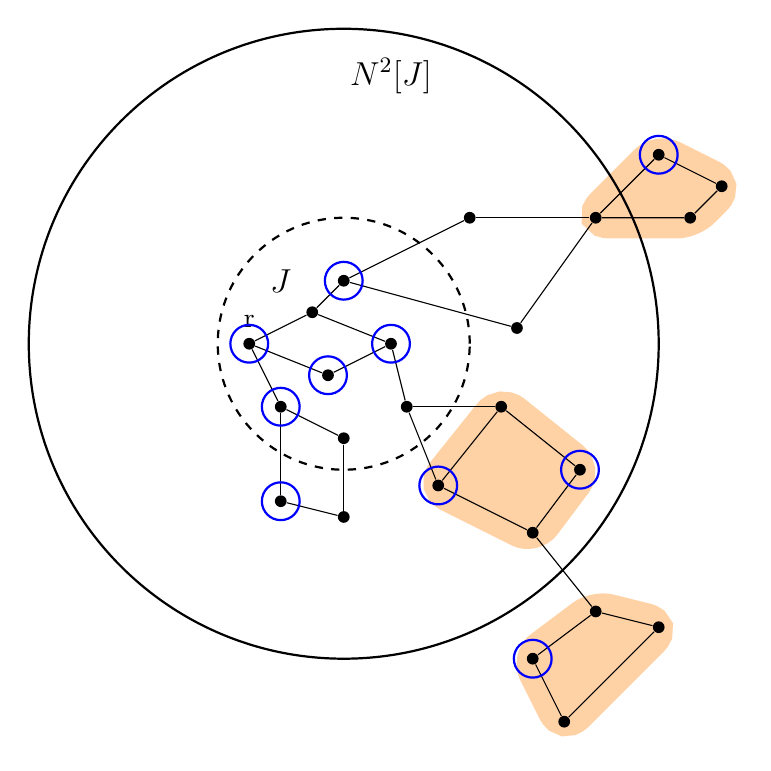
\begin{tikzpicture}[scale=0.8]
    
                %%%%%%%%%%%%%%%%%%%%%%%%%%%%%%%%%%%%%%%%%%%%%
                %%%%%%%%%%%%%%%%%%%%%%%%%%%%%%%%%%%%%%%%%%%%%
                %%%%%%%%%%%%%%%%%%%%%%%%%%%%%%%%%%%%%%%%%%%%%
                %%%%%%%%%%%%%%%%%%%%%%%%%%%%%%%%%%%%%%%%%%%%%
                %%%%%%%%%%%%%%%%%%%%%%%%%%%%%%%%%%%%%%%%%%%%%
                %%%%%%%%%%%%%%%%%%%%%%%%%%%%%%%%%%%%%%%%%%%%%
                %%%%%%%%%%%%%%%%%%%%%%%%%%%%%%%%%%%%%%%%%%%%%
                %%%%%%%%%%%%%%%%%%%%%%%%%%%%%%%%%%%%%%%%%%%%%
                %%%%%%%%%%%%%%%%%%%%%%%%%%%%%%%%%%%%%%%%%%%%%
                %%%%%%%%%%%%%%%%%%%%%%%%%%%%%%%%%%%%%%%%%%%%%
                %%%%%%%%%%%%%%%%%%%%%%%%%%%%%%%%%%%%%%%%%%%%%
                %%%%%%%%%%%%%%%%%%%%%%%%%%%%%%%%%%%%%%%%%%%%%
                
                %Draw J vertices
                \node[fill=black, circle, inner sep=1.5pt] (j01) at (0.75,0.5) {};
                \node[fill=black, circle, inner sep=1.5pt, label=above:r] (j02) at (-0.5,1) {};
                \node[fill=black, circle, inner sep=1.5pt] (j03) at (0.5,1.5) {};
                \node[fill=black, circle, inner sep=1.5pt] (j04) at (1.75,1) {};
    
                \node[fill=black, circle, inner sep=1.5pt] (j1) at (0,0) {};
                \node[fill=black, circle, inner sep=1.5pt] (j2) at (2,0) {};
                \node[fill=black, circle, inner sep=1.5pt] (j3) at (1,2) {};
                \node[fill=black, circle, inner sep=1.5pt] (j4) at (1,-0.5) {};
                
                % Draw N^1[J] vertices
    
                \node[fill=black, circle, inner sep=1.5pt] (n11) at (3.5,0) {};
                \node[fill=black, circle, inner sep=1.5pt] (n12) at (3.75,1.25) {};
                \node[fill=black, circle, inner sep=1.5pt] (n13) at (3,3) {};
                \node[fill=black, circle, inner sep=1.5pt] (n14) at (0,-1.5) {};
                \node[fill=black, circle, inner sep=1.5pt] (n15) at (1,-1.75) {};
                \node[fill=black, circle, inner sep=1.5pt] (n16) at (2.5,-1.25) {};
    
    
                % Draw N^2[J] vertices
                \node[fill=black, circle, inner sep=1.5pt] (n21) at (5, 3) {};
                \node[fill=black, circle, inner sep=1.5pt] (n22) at (4,-2) {};
                \node[fill=black, circle, inner sep=1.5pt] (n23) at (4.75,-1) {};
    
                % Draw vertices outside N^2[J]
                \node[fill=black, circle, inner sep=1.5pt] (n31) at (4, -4) {};
                \node[fill=black, circle, inner sep=1.5pt] (n32) at (5, -3.25) {};
                \node[fill=black, circle, inner sep=1.5pt] (n33) at (6, -3.5) {};
                \node[fill=black, circle, inner sep=1.5pt] (n34) at (4.5, -5) {};

                \node[fill=black, circle, inner sep=1.5pt] (new31) at (6, 4) {};
                \node[fill=black, circle, inner sep=1.5pt] (new32) at (6.5, 3) {};
                \node[fill=black, circle, inner sep=1.5pt] (new33) at (7, 3.5) {};
    
                % Draw edges inside J (induced subgraph)
                \draw (j01) -- (j02);
                \draw (j02) -- (j03);
                \draw (j03) -- (j04);
                \draw (j04) -- (j01);
    
                \draw (j4) -- (j1);

                \draw (j02) -- (j1);
                \draw (j04) -- (j2);
                \draw (j03) -- (j3);
                
                % Draw edges from J to N^1[J]
                \draw (j2) -- (n11);
                \draw (j2) -- (n16);
                \draw (j3) -- (n12);
                \draw (j1) -- (n14);
                \draw (j3) -- (n13);
                \draw (j4) -- (n15);
    
                % Draw edges inside N^1[J]
                \draw (n14) -- (n15);
                \draw (n16) -- (n11);
    
                % Draw edges between N^1[J] and N^2[J]
                \draw (n16) -- (n22);
                \draw (n11) -- (n23);
                \draw (n13) -- (n21);
                \draw (n12) -- (n21);
    
                % Draw edges between N^2[J] and N^2[J]
                \draw (n22) -- (n23);
    
                % Draw edges between N^2[J] and the other part of the graph
                \draw (n22) -- (n32);
    
                % Draw edges between the edges that are outside of N^2[J]
                \draw (n31) -- (n32);
                \draw (n32) -- (n33);
                \draw (n33) -- (n34);
                \draw (n34) -- (n31);

                \draw (n21) -- (new31);
                \draw (n21) -- (new32);
                \draw (new31) -- (new33);
                \draw (new32) -- (new33);
    
                % Draw the J circle
                \draw[dashed, thick] (1,1) circle [radius=2];
                \node at (0,2) {\large $J$};
    
                % Draw the N^2[J] boundary as a larger circle
                \draw[thick] (1,1) circle [radius=5];
                \node at (1.75,5.25) {\large $N^2[J]$};
    
                % Draw vertices that are part of S_1
                \draw[blue, thick] (j01) circle(0.3);
                \draw[blue, thick] (j02) circle(0.3);
                \draw[blue, thick] (j04) circle(0.3);
    
                \draw[blue, thick] (j1) circle(0.3);
                \draw[blue, thick] (j3) circle(0.3);
                \draw[blue, thick] (n14) circle(0.3);
                \draw[blue, thick] (n16) circle(0.3);
                \draw[blue, thick] (n23) circle(0.3);
                \draw[blue, thick] (n31) circle(0.3);
                \draw[blue, thick] (new31) circle(0.3);
    
                \begin{scope}[on background layer]   
                    \filldraw[orange!35,line width=15pt,rounded corners=5pt] (n31.center) -- (n32.center) -- (n33.center) -- (n34.center) -- cycle;
                \end{scope}
    
                \begin{scope}[on background layer]   
                    \filldraw[orange!35,line width=15pt,rounded corners=5pt] (n22.center) -- (n23.center) -- (n11.center) -- (n16.center) -- cycle;
                \end{scope}

                \begin{scope}[on background layer]   
                    \filldraw[orange!35,line width=15pt,rounded corners=5pt] (n21.center) -- (new31.center) -- (new33.center) -- (new32.center) -- cycle;
                \end{scope}
    
            \end{tikzpicture}
            \caption{$\forall v \in \{v_1,v_2,v_3,v_4\}: v \notin J$}
            \label{fig:second-figure}
        \end{minipage}
    \end{figure}


    \item $\exists v' \in \{v_1,v_2,v_3,v_4\}: v' \in J$. This also means that in this case 
    $\forall v' \in \{v_1,v_2,v_3,v_4\}: v' \in N^{2}_{G}[J]$.
    There are two cases to consider again. We know there $\exists v'' \in \{v_1,v_2,v_3,v_4\}$, 
    such that $v'' \in S_1$, we still have not considered whether or not it is a part of $J$.

    \begin{enumerate}
        \item $\exists v \in S_1: v \notin J$:
        
        In this case we can directly apply the previous point. From the properties of the set 
        difference operator we get: $v \in S_1 \backslash J \subseteq S_2 \oplus^{2}_{G,J} S_1$. 
        Consult Fig.~\ref{fig:third-figure} to see that there exists a vertex $v_{1,4}$ that is a part of 
        the 4-cycle, $v_{1,4} \notin J$, therefore $v_{1,4} \in S_1 \backslash J \subseteq S_2 \oplus^{2}_{G,J} S_1$.
        This means that in the new set $v_{1,4}$ will break that cycle.

        \item $\forall v \in S_1: v \in J$:

        In line~\ref{state:construct-H} of Algorithm~\ref{alg:stitch-fvs-4cl}, we have the following 
        construction of $H \leftarrow G[N^{2}_{G}[J] \backslash (S_1 \backslash J)]$. 

        \begin{align}
            V(H) &= N^{2}_{G}[J] \backslash (S_1 \backslash J) \\
                 &= N^{2}_{G}[J] \cap J \cup (N^{2}_G[J] \backslash S_1) \\
                 &= J \cup (N^{2}_G[J] \backslash S_1)
        \end{align}

        However, $\forall v \in \{v_1,v_2,v_3,v_4\}: v \in S_1 \land v \in J$. 
        Therefore $\{v_1,v_2,v_3,v_4\} \subseteq V(H)$. This means that in line~\ref{state:opt-solution} of 
        Algorithm~\ref{alg:stitch-fvs-4cl} we will add some $v^{*} \in \{v_1,v_2,v_3,v_4\}$ to $S_2$.

        Therefore $v \in S_2$, which has the same meaning as $v \in S_2 \cap N^{2}_{G}[J]$,
        and because $S_2 \cap N^{2}_{G}[J] \subseteq S_2 \oplus^{2}_{G,J} S_1$, we get 
        $v \in S_2 \oplus^{2}_{G,J} S_1$.

        Consult Fig.~\ref{fig:fourth-figure}. 

    \end{enumerate}

    \begin{figure}[H]
        \centering
        \begin{minipage}{0.50\textwidth}
            \centering
            \begin{tikzpicture}[scale=0.8]
                %Draw J vertices
                \node[fill=black, circle, inner sep=1.5pt] (j01) at (0.75,0.5) {};
                \node[fill=black, circle, inner sep=1.5pt, label=above:r] (j02) at (-0.5,1) {};
                \node[fill=black, circle, inner sep=1.5pt] (j03) at (0.5,1.5) {};
                \node[fill=black, circle, inner sep=1.5pt] (j04) at (1.75,1) {};
        
                \node[fill=black, circle, inner sep=1.5pt] (j1) at (0,0) {};
                \node[fill=black, circle, inner sep=1.5pt] (j2) at (2,0) {};
                \node[fill=black, circle, inner sep=1.5pt] (j3) at (1,2) {};
                \node[fill=black, circle, inner sep=1.5pt] (j4) at (1,-0.5) {};
                
                % Draw N^1[J] vertices
        
                \node[fill=black, circle, inner sep=1.5pt] (n11) at (3.5,0) {};
                \node[fill=black, circle, inner sep=1.5pt] (n12) at (3.75,1.25) {};
                \node[fill=black, circle, inner sep=1.5pt] (n13) at (3,3) {};
                \node[fill=black, circle, inner sep=1.5pt, label=below:$v_{1,4}$]  at (0,-1.5) {};
                \node[fill=black, circle, inner sep=1.5pt] (n15) at (1,-1.75) {};
                \node[fill=black, circle, inner sep=1.5pt] (n16) at (2.5,-1.25) {};
        
        
                % Draw N^2[J] vertices
                \node[fill=black, circle, inner sep=1.5pt] (n21) at (5, 3) {};
                \node[fill=black, circle, inner sep=1.5pt] (n22) at (4,-2) {};
                \node[fill=black, circle, inner sep=1.5pt] (n23) at (4.75,-1) {};
        
                % Draw vertices outside N^2[J]
                \node[fill=black, circle, inner sep=1.5pt] (n31) at (4, -4) {};
                \node[fill=black, circle, inner sep=1.5pt] (n32) at (5, -3.25) {};
                \node[fill=black, circle, inner sep=1.5pt] (n33) at (6, -3.5) {};
                \node[fill=black, circle, inner sep=1.5pt] (n34) at (4.5, -5) {};

                \node[fill=black, circle, inner sep=1.5pt] (new31) at (6, 4) {};
                \node[fill=black, circle, inner sep=1.5pt] (new32) at (6.5, 3) {};
                \node[fill=black, circle, inner sep=1.5pt] (new33) at (7, 3.5) {};

                % Draw edges inside J (induced subgraph)
                \draw (j01) -- (j02);
                \draw (j02) -- (j03);
                \draw (j03) -- (j04);
                \draw (j04) -- (j01);
        
                \draw (j4) -- (j1);

                \draw (j02) -- (j1);
                \draw (j04) -- (j2);
                \draw (j03) -- (j3);
                
                % Draw edges from J to N^1[J]
                \draw (j2) -- (n11);
                \draw (j2) -- (n16);
                \draw (j3) -- (n12);
                \draw (j1) -- (n14);
                \draw (j3) -- (n13);
                \draw (j4) -- (n15);
        
                % Draw edges inside N^1[J]
                \draw (n14) -- (n15);
                \draw (n16) -- (n11);
        
                % Draw edges between N^1[J] and N^2[J]
                \draw (n16) -- (n22);
                \draw (n11) -- (n23);
                \draw (n13) -- (n21);
                \draw (n12) -- (n21);
        
                % Draw edges between N^2[J] and N^2[J]
                \draw (n22) -- (n23);
        
                % Draw edges between N^2[J] and the other part of the graph
                \draw (n22) -- (n32);
        
                % Draw edges between the edges that are outside of N^2[J]
                \draw (n31) -- (n32);
                \draw (n32) -- (n33);
                \draw (n33) -- (n34);
                \draw (n34) -- (n31);

                \draw (n21) -- (new31);
                \draw (n21) -- (new32);
                \draw (new31) -- (new33);
                \draw (new32) -- (new33);
        
                % Draw the J circle
                \draw[dashed, thick] (1,1) circle [radius=2];
                \node at (0,2) {\large $J$};
        
                % Draw the N^2[J] boundary as a larger circle
                \draw[thick] (1,1) circle [radius=5];
                \node at (1.75,5.25) {\large $N^2[J]$};
        
                % Draw vertices that are part of S_1
                \draw[blue, thick] (j01) circle(0.3);
                \draw[blue, thick] (j02) circle(0.3);
                \draw[blue, thick] (j04) circle(0.3);
        
                \draw[blue, thick] (j1) circle(0.3);
                \draw[blue, thick] (j3) circle(0.3);
                \draw[blue, thick] (n14) circle(0.3);
                \draw[blue, thick] (n16) circle(0.3);
                \draw[blue, thick] (n23) circle(0.3);
                \draw[blue, thick] (n31) circle(0.3);
                \draw[blue, thick] (new31) circle(0.3);
    
                \begin{scope}[on background layer]   
                    \filldraw[orange!35,line width=15pt,rounded corners=5pt] (j1.center) -- (n14.center) -- (n15.center) -- (j4.center) -- cycle;
                \end{scope}
        
                %%%%%%%%%%%%%%%%%%%%%%%%%%%%%%%%%%%%%%%%%%%%%
                %%%%%%%%%%%%%%%%%%%%%%%%%%%%%%%%%%%%%%%%%%%%%
                %%%%%%%%%%%%%%%%%%%%%%%%%%%%%%%%%%%%%%%%%%%%%
                %%%%%%%%%%%%%%%%%%%%%%%%%%%%%%%%%%%%%%%%%%%%%
                %%%%%%%%%%%%%%%%%%%%%%%%%%%%%%%%%%%%%%%%%%%%%
                %%%%%%%%%%%%%%%%%%%%%%%%%%%%%%%%%%%%%%%%%%%%%
                %%%%%%%%%%%%%%%%%%%%%%%%%%%%%%%%%%%%%%%%%%%%%
                %%%%%%%%%%%%%%%%%%%%%%%%%%%%%%%%%%%%%%%%%%%%%
                %%%%%%%%%%%%%%%%%%%%%%%%%%%%%%%%%%%%%%%%%%%%%
                %%%%%%%%%%%%%%%%%%%%%%%%%%%%%%%%%%%%%%%%%%%%%
                %%%%%%%%%%%%%%%%%%%%%%%%%%%%%%%%%%%%%%%%%%%%%
                %%%%%%%%%%%%%%%%%%%%%%%%%%%%%%%%%%%%%%%%%%%%%
    
        
            \end{tikzpicture}
        \caption{$\exists v \in S_1: v \notin J$ (Remember we are in the case 
        where $\exists v \in J$)}
        \label{fig:third-figure}
        \end{minipage}
        \hfill
        \begin{minipage}{0.49\textwidth}
            \centering
            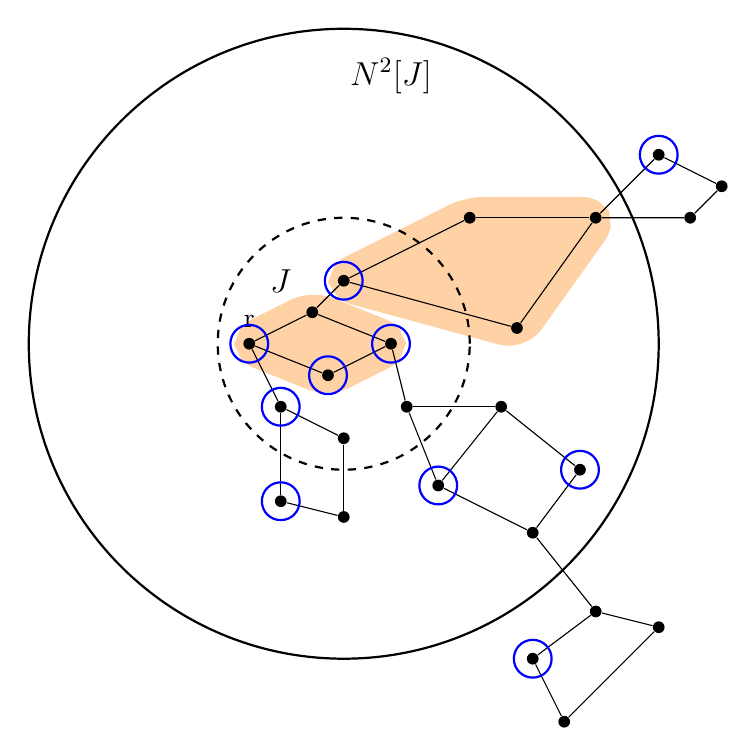
\begin{tikzpicture}[scale=0.8]
    
                %%%%%%%%%%%%%%%%%%%%%%%%%%%%%%%%%%%%%%%%%%%%%
                %%%%%%%%%%%%%%%%%%%%%%%%%%%%%%%%%%%%%%%%%%%%%
                %%%%%%%%%%%%%%%%%%%%%%%%%%%%%%%%%%%%%%%%%%%%%
                %%%%%%%%%%%%%%%%%%%%%%%%%%%%%%%%%%%%%%%%%%%%%
                %%%%%%%%%%%%%%%%%%%%%%%%%%%%%%%%%%%%%%%%%%%%%
                %%%%%%%%%%%%%%%%%%%%%%%%%%%%%%%%%%%%%%%%%%%%%
                %%%%%%%%%%%%%%%%%%%%%%%%%%%%%%%%%%%%%%%%%%%%%
                %%%%%%%%%%%%%%%%%%%%%%%%%%%%%%%%%%%%%%%%%%%%%
                %%%%%%%%%%%%%%%%%%%%%%%%%%%%%%%%%%%%%%%%%%%%%
                %%%%%%%%%%%%%%%%%%%%%%%%%%%%%%%%%%%%%%%%%%%%%
                %%%%%%%%%%%%%%%%%%%%%%%%%%%%%%%%%%%%%%%%%%%%%
                %%%%%%%%%%%%%%%%%%%%%%%%%%%%%%%%%%%%%%%%%%%%%
                
                %Draw J vertices
                \node[fill=black, circle, inner sep=1.5pt] (j01) at (0.75,0.5) {};
                \node[fill=black, circle, inner sep=1.5pt, label=above:r] (j02) at (-0.5,1) {};
                \node[fill=black, circle, inner sep=1.5pt] (j03) at (0.5,1.5) {};
                \node[fill=black, circle, inner sep=1.5pt] (j04) at (1.75,1) {};
    
                \node[fill=black, circle, inner sep=1.5pt] (j1) at (0,0) {};
                \node[fill=black, circle, inner sep=1.5pt] (j2) at (2,0) {};
                \node[fill=black, circle, inner sep=1.5pt] (j3) at (1,2) {};
                \node[fill=black, circle, inner sep=1.5pt] (j4) at (1,-0.5) {};
                
                % Draw N^1[J] vertices
    
                \node[fill=black, circle, inner sep=1.5pt] (n11) at (3.5,0) {};
                \node[fill=black, circle, inner sep=1.5pt] (n12) at (3.75,1.25) {};
                \node[fill=black, circle, inner sep=1.5pt] (n13) at (3,3) {};
                \node[fill=black, circle, inner sep=1.5pt] (n14) at (0,-1.5) {};
                \node[fill=black, circle, inner sep=1.5pt] (n15) at (1,-1.75) {};
                \node[fill=black, circle, inner sep=1.5pt] (n16) at (2.5,-1.25) {};
    
    
                % Draw N^2[J] vertices
                \node[fill=black, circle, inner sep=1.5pt] (n21) at (5, 3) {};
                \node[fill=black, circle, inner sep=1.5pt] (n22) at (4,-2) {};
                \node[fill=black, circle, inner sep=1.5pt] (n23) at (4.75,-1) {};
    
                % Draw vertices outside N^2[J]
                \node[fill=black, circle, inner sep=1.5pt] (n31) at (4, -4) {};
                \node[fill=black, circle, inner sep=1.5pt] (n32) at (5, -3.25) {};
                \node[fill=black, circle, inner sep=1.5pt] (n33) at (6, -3.5) {};
                \node[fill=black, circle, inner sep=1.5pt] (n34) at (4.5, -5) {};

                \node[fill=black, circle, inner sep=1.5pt] (new31) at (6, 4) {};
                \node[fill=black, circle, inner sep=1.5pt] (new32) at (6.5, 3) {};
                \node[fill=black, circle, inner sep=1.5pt] (new33) at (7, 3.5) {};
    
                % Draw edges inside J (induced subgraph)
                \draw (j01) -- (j02);
                \draw (j02) -- (j03);
                \draw (j03) -- (j04);
                \draw (j04) -- (j01);
    
                \draw (j4) -- (j1);

                \draw (j02) -- (j1);
                \draw (j04) -- (j2);
                \draw (j03) -- (j3);
                
                % Draw edges from J to N^1[J]
                \draw (j2) -- (n11);
                \draw (j2) -- (n16);
                \draw (j3) -- (n12);
                \draw (j1) -- (n14);
                \draw (j3) -- (n13);
                \draw (j4) -- (n15);
    
                % Draw edges inside N^1[J]
                \draw (n14) -- (n15);
                \draw (n16) -- (n11);
    
                % Draw edges between N^1[J] and N^2[J]
                \draw (n16) -- (n22);
                \draw (n11) -- (n23);
                \draw (n13) -- (n21);
                \draw (n12) -- (n21);
    
                % Draw edges between N^2[J] and N^2[J]
                \draw (n22) -- (n23);
    
                % Draw edges between N^2[J] and the other part of the graph
                \draw (n22) -- (n32);
    
                % Draw edges between the edges that are outside of N^2[J]
                \draw (n31) -- (n32);
                \draw (n32) -- (n33);
                \draw (n33) -- (n34);
                \draw (n34) -- (n31);

                \draw (n21) -- (new31);
                \draw (n21) -- (new32);
                \draw (new31) -- (new33);
                \draw (new32) -- (new33);
    
                % Draw the J circle
                \draw[dashed, thick] (1,1) circle [radius=2];
                \node at (0,2) {\large $J$};
    
                % Draw the N^2[J] boundary as a larger circle
                \draw[thick] (1,1) circle [radius=5];
                \node at (1.75,5.25) {\large $N^2[J]$};
    
                % Draw vertices that are part of S_1
                \draw[blue, thick] (j01) circle(0.3);
                \draw[blue, thick] (j02) circle(0.3);
                \draw[blue, thick] (j04) circle(0.3);
    
                \draw[blue, thick] (j1) circle(0.3);
                \draw[blue, thick] (j3) circle(0.3);
                \draw[blue, thick] (n14) circle(0.3);
                \draw[blue, thick] (n16) circle(0.3);
                \draw[blue, thick] (n23) circle(0.3);
                \draw[blue, thick] (n31) circle(0.3);
                \draw[blue, thick] (new31) circle(0.3);
    
                \begin{scope}[on background layer]   
                    \filldraw[orange!35,line width=15pt,rounded corners=5pt] (j01.center) -- (j02.center) -- (j03.center) -- (j04.center) -- cycle;
                \end{scope}
    
                \begin{scope}[on background layer]   
                    \filldraw[orange!35,line width=15pt,rounded corners=5pt] (j3.center) -- (n12.center) -- (n21.center) -- (n13.center) -- cycle;
                \end{scope}
    
            \end{tikzpicture}
            \caption{$\forall v \in S_1: v \in J$}
            \label{fig:fourth-figure}
        \end{minipage}
    \end{figure}

\end{enumerate}

 The proof of optimality of the set $S_2 \oplus^{2}_{G,J} S_1$ is similar to the one in 
Bumpus et al.\cite[Lemma 3.2]{bumpus_et_al:LIPIcs.SWAT.2024.19}. It is important to note 
that we can use the same proof, because of a property of the FVS-4CL problem, namely that 
a 4-cycle breaking set is closed under taking induced subgraphs.

 Remember, we are still trying to prove what we mentioned in Algorithm~\ref{alg:p-m-stitching},
namely that some feasible solution $S'$ (which in our case is the $S_2 \oplus^{2}_{G,J} S_1$), is of minimum weight,
that is, for all other feasible solutions $S^{*}$, it holds that $w(S') \leq w(S^{*} \oplus^{2}_{G,J} S_1)$.

Assume by way of contradiction that there is a feasible solution $S_3$ for $G$,
such that $w(S_3 \oplus^{2}_{G,J} S_1) < w(S_2 \oplus^{2}_{G,J} S_1)$. Then it would follow that:

\[
\begin{aligned}
w|_{V(F)}(S_2) &= w(S_2) && \text{since } S_2 \subseteq V(F) \text{} \\
&= w(S_2 \cap N^{2}_{G}[J]) && \text{since } V(F) \subseteq N^{2}_{G}[J] \\
&= w(S_1 \setminus J) + w(S_2 \cap N^{2}_{G}[J]) - w(S_1 \setminus J)  \\
&= w((S_1 \setminus J) \cup (S_2 \cap N^{2}_{G}[J])) - w(S_1 \setminus J) && \text{since } V(F) \cap (S_1 \setminus J) = \emptyset \\
&= w(S_2 \oplus^{2}_{G,J} S_1) - w(S_1 \setminus J) && \text{by definition of stitch} \\
&> w(S_3 \oplus^{2}_{G,J} S_1) - w(S_1 \setminus J) && \text{by assumption on } S_3 \\
&= w((S_1 \setminus J) \cup (S_3 \cap N^{2}_{G}[J])) - w(S_1 \setminus J) && \text{by definition of stitch} \\
&= w((S_3 \cap N^{2}_{G}[J]) \setminus (S_1 \setminus J)) && \text{since } w(A \cup B) - w(A) = w(B \setminus A)  \\
&= w(S_3 \cap (N^{2}_{G}[J] \setminus (S_1 \setminus J))) && \text{since } (A \cap B) \setminus C = A \cap (B \setminus C)  \\
&= w(S_3 \cap V(F)) && \text{by definition of } F \\
&= w|_{V(F)}(S_3 \cap V(F))
\end{aligned}
\]
\end{proof}

\textbf{Running time:}

The running time of the algorithm is dominated by the call of algorithm $A$. For 
$\tw$, the treewidth of $N^{2}_{G}[J]$, 
the running time is 
$2^{\mathcal{O}(\tw^2)} \cdot n^{\mathcal{O}(1)}$. Here we use the dynamic programming algorithm (\ref{alg:dp}).

\subsection{FVS-BCL and ($\rho / 2$)-stitching}

In this subsection, we extend the results for FVS-4CL to the more general problem. 
In earlier sections, we showed that FVS-BCL admits an EPTAS by observing that 
$\lfloor \frac{\rho}{2} \rfloor$ layers of overlap between two subgraphs are sufficient for a 
$\rho$-cycle to be entirely contained within one of the subgraphs, possibly including the 
overlapping region (see Fig.~\ref{fig:bfs_tree}, \ref{fig:first-figure}). 
When applying the $m$-stitching technique, the reader should understand that the two relevant 
subgraphs are $G[V(G) \setminus J]$ and $G[J]$. If we construct an algorithm similar to 
Algorithm~\ref{alg:stitch-fvs-4cl} but set the parameter $m$ to 
$\lfloor \frac{\rho}{2} \rfloor$ instead of 2, the resulting algorithm solves 
FVS-BCL-stitching in time 
$f(\tw) \cdot n^{\mathcal{O}(1)}$ 
where $\tw$ is the treewidth of $N^{\lfloor\frac{\rho}{2}\rfloor}_{G}[J]$. 
It is important to note that a $\rho$-cycle breaking set is closed under taking 
induced subgraphs. This is another reason we can construct such an algorithm and do not 
have to take a different approach as we will do with the $r$-Dominating Set.

From the arguments in the previous paragraph we can infer that:

\begin{enumerate}
    \item FVS-BCL is $\lfloor\frac{\rho}{2}\rfloor$-stitchable.
    \item There exists an algorithm $A_{\text{FVS-BCL}}$ which solves 
    FVS-BCL-$\lfloor\frac{\rho}{2}\rfloor$-stitching in time 
    $f(\tw) \cdot n^{\mathcal{O}(1)}$ 
    where $\tw$ is the treewidth of any $N^{\lfloor\frac{\rho}{2}\rfloor}_{G}[J]$ and 
    $f$ is some computable function.
\end{enumerate}

The problem is also trivially guessable. Like in the FVS-4CL, taking the set $V(G)$, would 
break all $\rho$-cycles in a graph.

\textbf{Running time:}

For some computable function $f$, constant $\rho$ and $\tw$, treewidth of 
$N^{\lfloor\frac{\rho}{2}\rfloor}_{G}[J]$,
the algorithm we described solves 
FVS-BCL-$\rho$-stitching in time $f(\tw) \cdot n^{\mathcal{O}(1)}$.

\subsection{r-Dominating Set and $(r+1)$-stitching}

In this subsection we will use the definitions and terminology we have established in the 
previous section and look at another problem, namely the r-Dominating Set problem. We will 
argue that in the case of that problem the parameter $m$ has to be set to $r+1$ in order 
to maintain feasibility when constructing new sets. Afterwards we will prove that 
when constructing new sets, one can find a feasible solution which is also optimal. 
We follow the steps we established in the previous section.

Firstly, prove that the problem is guessable and m-stitchable. Secondly, devise an algorithm 
$A_{\text{r-DS}}$ that solves the problem in FPT. Finally, using Theorem~\ref{theorem-main}, 
prove that the problem is certified.

\refstepcounter{definition}
\begin{mydefinition}[\boldsymbol{$r$}-DS is guessable]{Lemma}
    \label{lemma-ds-guessable}

    For any planar graph $G$, the set $V(G)$ is a feasible solution to r-DS.

\end{mydefinition}

\begin{proof}
    Let $X$ be the set of all vertices in $G$, $X \leftarrow V(G)$. Therefore, it is 
    trivially true that $N^r_G[X] = V(G)$. 
\end{proof}

\refstepcounter{definition}
\begin{mydefinition}[r-DS is $(r+1)$-stitchable]{Lemma}
    \label{lemma-r-DS-stitchable}

    Let $(G, w)$ be any instance to the $r$-DS problem, $J \subseteq V(G)$, some subset
    of the vertices in the graph 
    and $S_1$ and $S_2$ any two feasible solutions to the problem in $G$. Then the set $S_3$:
    \[S_3 := (S_1 \backslash J) \cup (S_2 \cap N^{r+1}_{G} \left[J\right]).\]
    is a feasible solution to the problem.

\end{mydefinition}

\begin{proof}
    For a vertex $v \in V(G)$, we have the following cases:

    \begin{enumerate}
        \item $v \in V(G) \backslash N^{r+1}_{G}[J]$. Because $S_1$ is a feasible solution,
        it is clear that $v$ will be dominated by some vertex $u$ in $S_1 \backslash J$. Since 
        $S_1 \backslash J \subseteq S_3$, then $u \in S_3$.
        \item $v \in N^{r+1}_{G}[J]$. Because $S_2$ is a feasible solution, it is clear 
        that $S_2 \cap N^{r+1}_{G}[J]$ contains a vertex $u$ which dominates $v$. Since 
        $S_2 \cap N^{r+1}_{G}[J] \subseteq S_3$, then $u \in S_3$.
    \end{enumerate}

    In both cases we have argued that there $\exists u \in S_3$, such that for any vertex 
    $v \in V(G)$, $u$ dominates $v$.

\end{proof}

Now we describe an algorithm to find a feasible solution of minimum weight.

\begin{algorithm}[H]
    \caption{Stitch-r-DS}
    \label{alg:stitch-r-DS}
    \begin{algorithmic}[1]
    \REQUIRE Vertex-weighted planar graph $(G, w:V(G) \to \mathbb{N})$,
    a feasible solution of r-DS $S_1$ on $G$
    and a vertex set $J \subseteq V(G)$.
    \ENSURE a feasible solution $S'$ on $G$, such that for all other feasible solutions $S^{*}$, 
    we have $w(S') \leq w(S^{*} \oplus^{r+1}_{G,J} S_1)$. 
    \STATE Let $H \leftarrow G[N^{r+1}_{G}[J]] \cup \{q\}$, where for vertex $q$
    it holds that $N_H(q) := N_{G}(N^{r}_{G}[J])$ (Vertex $q$ is adjacent to the vertices 
    at distance exactly $r+1$ from $J$). \label{state:construct-H-rds}
    \STATE \[
    w_H(x) = 
    \begin{cases}
    0 & \text{if } x \in (S_1 \setminus J) \cup \{q\} \\
    w(x) & \text{otherwise}
    \end{cases}
    \]
    \STATE Let $S_2'$ be the output of algorithm $A$ on input $(H, w)$. 
    \STATE Let $S_2 = S_2' \backslash \{q\}$. \label{state:opt-solution-rds}
    \IF{ $w(S_2 \oplus^{r+1}_{G,J} S_1) < w(S_1)$ }
        \RETURN $S_2 \oplus^{r+1}_{G,J} S_1$
    \ELSE
        \RETURN $S_1$
    \ENDIF
    \end{algorithmic}
\end{algorithm}

\refstepcounter{definition}
\begin{mydefinition}[$r$-DS-$(r+1)$-stitching]{Lemma}
    \label{lemma-rds-stitching}

    Let $A$ be an algorithm that solves $r$-stitching on any vertex-weighted instance 
    $(G, w : V(G) \to \mathbb{N})$ in time $f(t) \cdot |V(G)|^{\mathcal{O}(1)}$ where 
    $t$ is the treewidth of $G$. Then 
    Algorithm~\ref{alg:stitch-r-DS} solves $r$-DS in time 
    $f(\tw) \cdot V(G)^{\mathcal{O}(1)}$ where $\tw$ is the treewidth of $(N^{r+1}_{G}[J])$.

\end{mydefinition}

The proof of Lemma~\ref{lemma-rds-stitching} is outside of the scope of this paper 
as it is similar to the proof of Lemma~\ref{lemma-stictch-fvs-4cl}. The reader can find 
a similar proof in Bumpus et al. \cite[Lemma 3.3]{bumpus_et_al:LIPIcs.SWAT.2024.19}.

\textbf{Running time:}

For some constant $r$ and $\tw$, the treewidth of $N^{r+1}_{G}[J]$, the running time of 
the algorithm is: $(2r+1)^{\tw + 1} \cdot \tw^{2} \cdot n^{\mathcal{O}(1)}$.
\section{Certified Algorithm}

In this section we initiate the study of certified algorithms for FVS-4CL and the more general 
FVS-BCL. In the final subsection the focus is shifted to the r-Dominating Set problem.



\subsection{FVS-4CL}





In the second stage, we compute a feasible solution $S$, set 
$J_\kappa$\footnote{
    A word on the argument $\kappa$ and the value that we set it to. In our case, for the FVS-4CL problem, 
    $m$ is equal to two. Also, $k = \lceil \frac{2m}{\epsilon} \rceil + 2m \geq 5$. Notice that the set 
    $J_{\kappa}$ is of width $k-2m$, therefore the $m$-neighbourhood (2-neighbourhood) is of width 
    $k - 2m + 2m = k$. Therefore, in our case, the graphs within we stitch are of width
    $k = \lceil \frac{2m}{\epsilon} \rceil + 2m \geq 5$.
    Take for example 
    vertex $v_{2,1}$ in Fig.~\ref{fig:reconfigure}. In order to find every cycle that it is a part of, 
    one would need to consider the layer that it is in, two layers to the left and two layers to the right. 

    \begin{figure}[H]
        \centering
        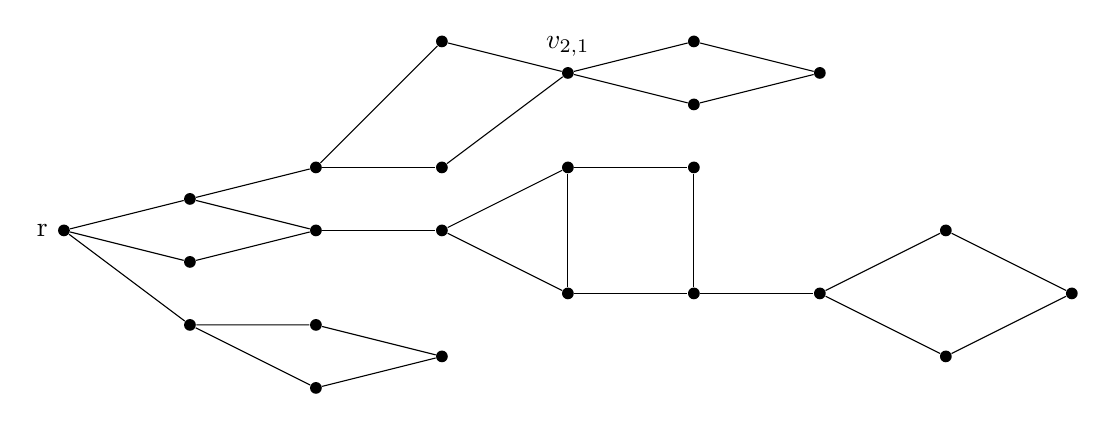
\begin{tikzpicture}[scale=0.8]
    
            \node[fill=black, circle, inner sep=1.5pt, label=left:r] (j02) at (-5,-1) {};
    
            \node[fill=black, circle, inner sep=1.5pt] (j1) at (-3,-2.5) {};
            \node[fill=black, circle, inner sep=1.5pt] (j01) at (-3,-1.5) {};
            \node[fill=black, circle, inner sep=1.5pt] (j03) at (-3,-0.5) {};
    
            \node[fill=black, circle, inner sep=1.5pt] (j04) at (-1,-1) {};
            \node[fill=black, circle, inner sep=1.5pt] (j3) at (-1,0) {};
            \node[fill=black, circle, inner sep=1.5pt] (j4) at (-1,-2.5) {};
            \node[fill=black, circle, inner sep=1.5pt] (n14) at (-1,-3.5) {};
    
    
    
            \node[fill=black, circle, inner sep=1.5pt] (j2) at (1,-1) {};
            \node[fill=black, circle, inner sep=1.5pt] (n12) at (1,2) {};
            \node[fill=black, circle, inner sep=1.5pt] (n13) at (1,0) {};
            \node[fill=black, circle, inner sep=1.5pt] (n15) at (1,-3) {};
    
            \node[fill=black, circle, inner sep=1.5pt] (n11) at (3,0) {};
            \node[fill=black, circle, inner sep=1.5pt] (n16) at (3,-2) {};
    
            \node[fill=black, circle, inner sep=1.5pt, label=above:$v_{2,1}$] (n21) at (3, 1.5) {};
            
            \node[fill=black, circle, inner sep=1.5pt] (n22) at (5,-2) {};
            \node[fill=black, circle, inner sep=1.5pt] (n23) at (5,0) {};
            \node[fill=black, circle, inner sep=1.5pt] (new31) at (5, 2) {};
            \node[fill=black, circle, inner sep=1.5pt] (new32) at (5, 1) {};
    
            \node[fill=black, circle, inner sep=1.5pt] (n32) at (7, -2) {};
            \node[fill=black, circle, inner sep=1.5pt] (new33) at (7,1.5) {};
    
    
            \node[fill=black, circle, inner sep=1.5pt] (n31) at (9, -3) {};
            \node[fill=black, circle, inner sep=1.5pt] (n33) at (9, -1) {};
    
    
            \node[fill=black, circle, inner sep=1.5pt] (n34) at (11, -2) {};
    
            % Draw edges inside J (induced subgraph)
            \draw (j01) -- (j02);
            \draw (j02) -- (j03);
            \draw (j03) -- (j04);
            \draw (j04) -- (j01);
    
            \draw (j4) -- (j1);
    
            \draw (j02) -- (j1);
            \draw (j04) -- (j2);
            \draw (j03) -- (j3);
            
            % Draw edges from J to N^1[J]
            \draw (j2) -- (n11);
            \draw (j2) -- (n16);
            \draw (j3) -- (n12);
            \draw (j1) -- (n14);
            \draw (j3) -- (n13);
            \draw (j4) -- (n15);
    
            % Draw edges inside N^1[J]
            \draw (n14) -- (n15);
            \draw (n16) -- (n11);
    
            % Draw edges between N^1[J] and N^2[J]
            \draw (n16) -- (n22);
            \draw (n11) -- (n23);
            \draw (n13) -- (n21);
            \draw (n12) -- (n21);
    
            % Draw edges between N^2[J] and N^2[J]
            \draw (n22) -- (n23);
    
            % Draw edges between N^2[J] and the other part of the graph
            \draw (n22) -- (n32);
    
            % Draw edges between the edges that are outside of N^2[J]
            \draw (n31) -- (n32);
            \draw (n32) -- (n33);
            \draw (n33) -- (n34);
            \draw (n34) -- (n31);
    
            \draw (n21) -- (new31);
            \draw (n21) -- (new32);
            \draw (new31) -- (new33);
            \draw (new32) -- (new33);
    
    
        \end{tikzpicture}
        \caption{Layer decomposition of graph in Fig.~\ref{fig:first-figure}}
        \label{fig:reconfigure}
    \end{figure}
}

\subsection{FVS-BCL}


\subsection{r-Dominating Set}

%\section{Conclusion}
This section introduces the topic and provides background information. 

\printbibliography

\end{document}
